% =============================================================================
%  Systémová príručka – Záhrada stratených ciest
%  Autor: Mykyta Olym, Počítačová grafika 2026/2027
% =============================================================================
\documentclass[11pt, a4paper]{article}
\newcommand{\druhprirucky}{Systémová príručka}
% =============================================================================
%  Spoločné nastavenie všetkých troch dokumentov (preklad: latexmk -xelatex)
%  Záhrada stratených ciest – izometrické bludisko v knihe, Mykyta Olym, PG 2026/2027
% =============================================================================

% ---------------------------------------------------------------- údaje projektu
\newcommand{\nazovprojektu}{Záhrada stratených ciest}
\newcommand{\podnazovprojektu}{izometrické bludisko v knihe}
\newcommand{\predmet}{Počítačová grafika}
\newcommand{\skolskyrok}{2026/2027}
\newcommand{\ucitel}{Course Instructor}
\newcommand{\autor}{Mykyta Olym}
\newcommand{\verzia}{2.0}

% ---------------------------------------------------------------- jazyk a písmo
\usepackage{fontspec}
\usepackage{polyglossia}
\setdefaultlanguage{slovak}
\setmainfont{TeX Gyre Pagella}
\setsansfont{TeX Gyre Heros}
% neproporcionálne písmo zo šablóny KPI (priečinok fonts/)
\setmonofont{SourceCodePro}[
  Path = fonts/, Extension = .otf, Scale = 0.85,
  UprightFont = *-Regular, BoldFont = *-Bold,
  ItalicFont = *-Italic, BoldItalicFont = *-BoldItalic]

% ---------------------------------------------------------------- strana
\usepackage[a4paper, top=25mm, bottom=30mm, left=28mm, right=25mm]{geometry}
\usepackage{fancyhdr}
\pagestyle{fancy}
\fancyhf{}
\fancyhead[L]{\small\nazovprojektu}
\fancyhead[R]{\small\druhprirucky}
\fancyfoot[R]{\thepage}
\renewcommand{\headrulewidth}{0.4pt}
\setlength{\headheight}{14pt}
\setlength{\parindent}{0pt}
\setlength{\parskip}{0.55em}
\setlength{\emergencystretch}{3em}   % dlhé názvy radšej zalomiť než vytlačiť za okraj
% názvy súborov sa smú zalomiť za lomkou, bodkou alebo podčiarknutím
\usepackage[hyphens]{url}
\newcommand{\subor}[1]{\nolinkurl{#1}}

% ---------------------------------------------------------------- obsah, obrázky, tabuľky
\usepackage{graphicx}
\graphicspath{{obrazky/}}
\usepackage{booktabs, tabularx, array, longtable}
\usepackage{float}
\usepackage[font=small, labelfont=bf]{caption}
\usepackage{enumitem}
\setlist{itemsep=0.15em, topsep=0.3em}
\usepackage{xcolor}
\usepackage{csquotes}
\usepackage[style=iso-numeric, backend=biber, sorting=none]{biblatex}
\addbibresource{literatura.bib}
\usepackage[hidelinks]{hyperref}

% ---------------------------------------------------------------- titulná strana podľa pokynov
\newcommand{\titulnastrana}{%
  \begin{titlepage}
    \centering
    {\large Katedra počítačov a informatiky\\
      Fakulta elektrotechniky a informatiky\\
      Technická univerzita v Košiciach\par}
    \vspace*{\fill}
    {\Huge\bfseries \nazovprojektu\par}
    \vspace{0.4em}
    {\large \podnazovprojektu\par}
    \vspace{1.2em}
    {\Large \predmet\par}
    \vspace{3em}
    {\LARGE \druhprirucky\par}
    \vspace*{\fill}
    \begin{minipage}[t]{0.62\textwidth}
      \raggedright
      \begin{tabular}{@{}ll@{}}
        Šk. rok:       & \skolskyrok \\
        Meno učiteľa:  & \ucitel
      \end{tabular}
    \end{minipage}%
    \begin{minipage}[t]{0.38\textwidth}
      \raggedleft
      \begin{tabular}{@{}ll@{}}
        Autori: & \autor
      \end{tabular}
    \end{minipage}
  \end{titlepage}
  \setcounter{page}{1}%
}

% Obsah je podľa pokynov kapitola 1, preto skutočné kapitoly začínajú číslom 2.
\newcommand{\obsah}{%
  \renewcommand{\contentsname}{1\quad Obsah}%
  \tableofcontents
  \setcounter{section}{1}%
  \clearpage
}

\usepackage{amsmath}

\begin{document}
\titulnastrana
\obsah

% =============================================================================
\section{Funkcia programu}

Záhrada stratených ciest je webová aplikácia – hra o~bludisku rozprávaná ako kniha. Menu aj
rozprávač príbehu je kniha na stole (HTML a CSS), herný svet je izometrická (presnejšie
dimetrická) kresba usadlosti pri rieke s~náhodne generovaným bludiskom zo živých plotov
uprostred (WebGL cez knižnicu Phaser). Program
\begin{itemize}
  \item vygeneruje dokonalé bludisko (medzi každými dvoma miestnosťami vedie práve jedna cesta)
    a rozmiestni v~ňom tri zväzky kresieb,
  \item nakreslí svet z~hotových kresieb (dlaždíc) izometrickou projekciou a maliarovým algoritmom,
    vynásobí ho s~textúrou papiera a vzdialené časti zosvetlí,
  \item hľadá najkratšiu cestu algoritmom A* pre chôdzu kliknutím, nápovedu, ukážku riešenia
    a pre chodcov po cestách dediny,
  \item riadi filmové scény: plynulý let kamery z~knihy do kresby a späť (kamera knihy aj kamera
    sveta sa riadia jedným časom), rozhovory, titulky, oslavu v~cieli,
  \item animuje knihu (otvorenie dosky, otáčanie listov v~3D, písanie textu), postavu, ľudí,
    zvieratá, vodu, rastliny vo vetre, dážď a vtáky,
  \item meria čas a kroky, riadi záložku (pauzu), nastavenia a zvuky.
\end{itemize}
Používanie programu opisuje samostatný dokument Používateľská príručka.

% =============================================================================
\section{Popis programu}

\subsection{Popis riešenia}

\subsubsection{Architektúra a použité knižnice}

Program je napísaný v~jazyku JavaScript (moduly ES) a beží v~prehliadači. Pri návrhu sa dodržali
pravidlá z~pokynov k~zadaniu~\cite{Pokyny}: titulná strana knihy (prvá strana po otvorení) uvádza
meno autora, katedru, fakultu, univerzitu, predmet a školský rok, strana O~knihe údaje o~projekte
a všetky nevratné akcie (zahodenie rozohranej cesty, návrat na obsah počas hry, zavretie knihy)
sa vykonajú až po potvrdení priamo na strane knihy.

Aplikácia má dve vrstvy:
\begin{itemize}
  \item \textbf{kniha na stole} – prvky HTML nad plátnom hry. Strany sa vytvoria zo šablón
    \subor{<template>} v~\subor{index.html}; doska, listy a kamera knihy sa animujú transformáciami
    CSS v~3D~\cite{MdnTransforms} a rozhraním Web Animations~\cite{MdnWaapi};
  \item \textbf{svet} – plátno WebGL, ktoré kreslí knižnica \textbf{Phaser 4.2.1}~\cite{Phaser}
    (scény, kamera, obrázky, animácie, častice, zvuk, vstup). Generovanie bludiska a hľadanie cesty
    zabezpečuje knižnica \textbf{rot.js 2.2.1}~\cite{RotJs} (\subor{ROT.Map.IceyMaze},
    \subor{ROT.Path.AStar}, generátor náhodných čísel so semienkom).
\end{itemize}
Obe vrstvy spája režisér (\subor{director.js}) – scenár celej aplikácie zapísaný ako postupnosť
asynchrónnych krokov (\subor{await}), podobne ako scenár filmu. Kým je na obrazovke kniha,
herná slučka Phaseru spí, takže kniha má celý výkon počítača.

Všetky kresby, zvuky a písma sú prevzaté (tabuľka~\ref{tab:zdroje}); nástroje v~priečinku
\subor{nastroje} z~nich pripravia atlas textúr a textúry knihy.

\begin{table}[H]
  \centering
  \caption{Prevzaté kresby, zvuky a písma}\label{tab:zdroje}
  \begin{tabularx}{\textwidth}{@{}>{\raggedright}p{0.36\textwidth}X@{}}
    \toprule
    \textbf{Zdroj} & \textbf{Použitie} \\ \midrule
    city game tileset~\cite{CityTileset} & všetky kresby sveta: terén, živé ploty, stavby, rastliny, postavy, zvieratá, voda, zväzok kresieb \\
    Everyone is Afraid to be Forgotten~\cite{Comigo} & bublina rozhovoru, kvapka dažďa, vlnka, vták, kurzor \\
    EPIC-Collection book~\cite{Melle} & otvorená kniha, predná doska, krúžky väzby \\
    Paper-Textures~\cite{Leschge}, Wood Table 001~\cite{PolyHaven} & papier sveta, stôl \\
    Hand Drawn Icon Pack~\cite{Limofeus}, Doodle Icons~\cite{Doodle}, Footprints~\cite{Footprints} & políčko, krúžok, fajka, čiara, záložka, stopa \\
    \cite{CynicPiano, Catmint, BirdsWind, RainSound, StreamSound, Footsteps, PencilSounds, Kenney} & hudba knihy a záhrady, vtáky, dážď, potok, kroky, ceruzka, zvuky knihy, bublinka, melódia \\
    ElevenLabs~\cite{ElevenLabs} & hlasy rozprávača a postáv (syntéza reči) \\
    Caveat~\cite{Caveat}, Cormorant~\cite{Cormorant} & písmo rukopisu a knižné písmo \\ \bottomrule
  \end{tabularx}
\end{table}

\subsubsection{Diagram použitia}

\begin{figure}[H]
  \centering
  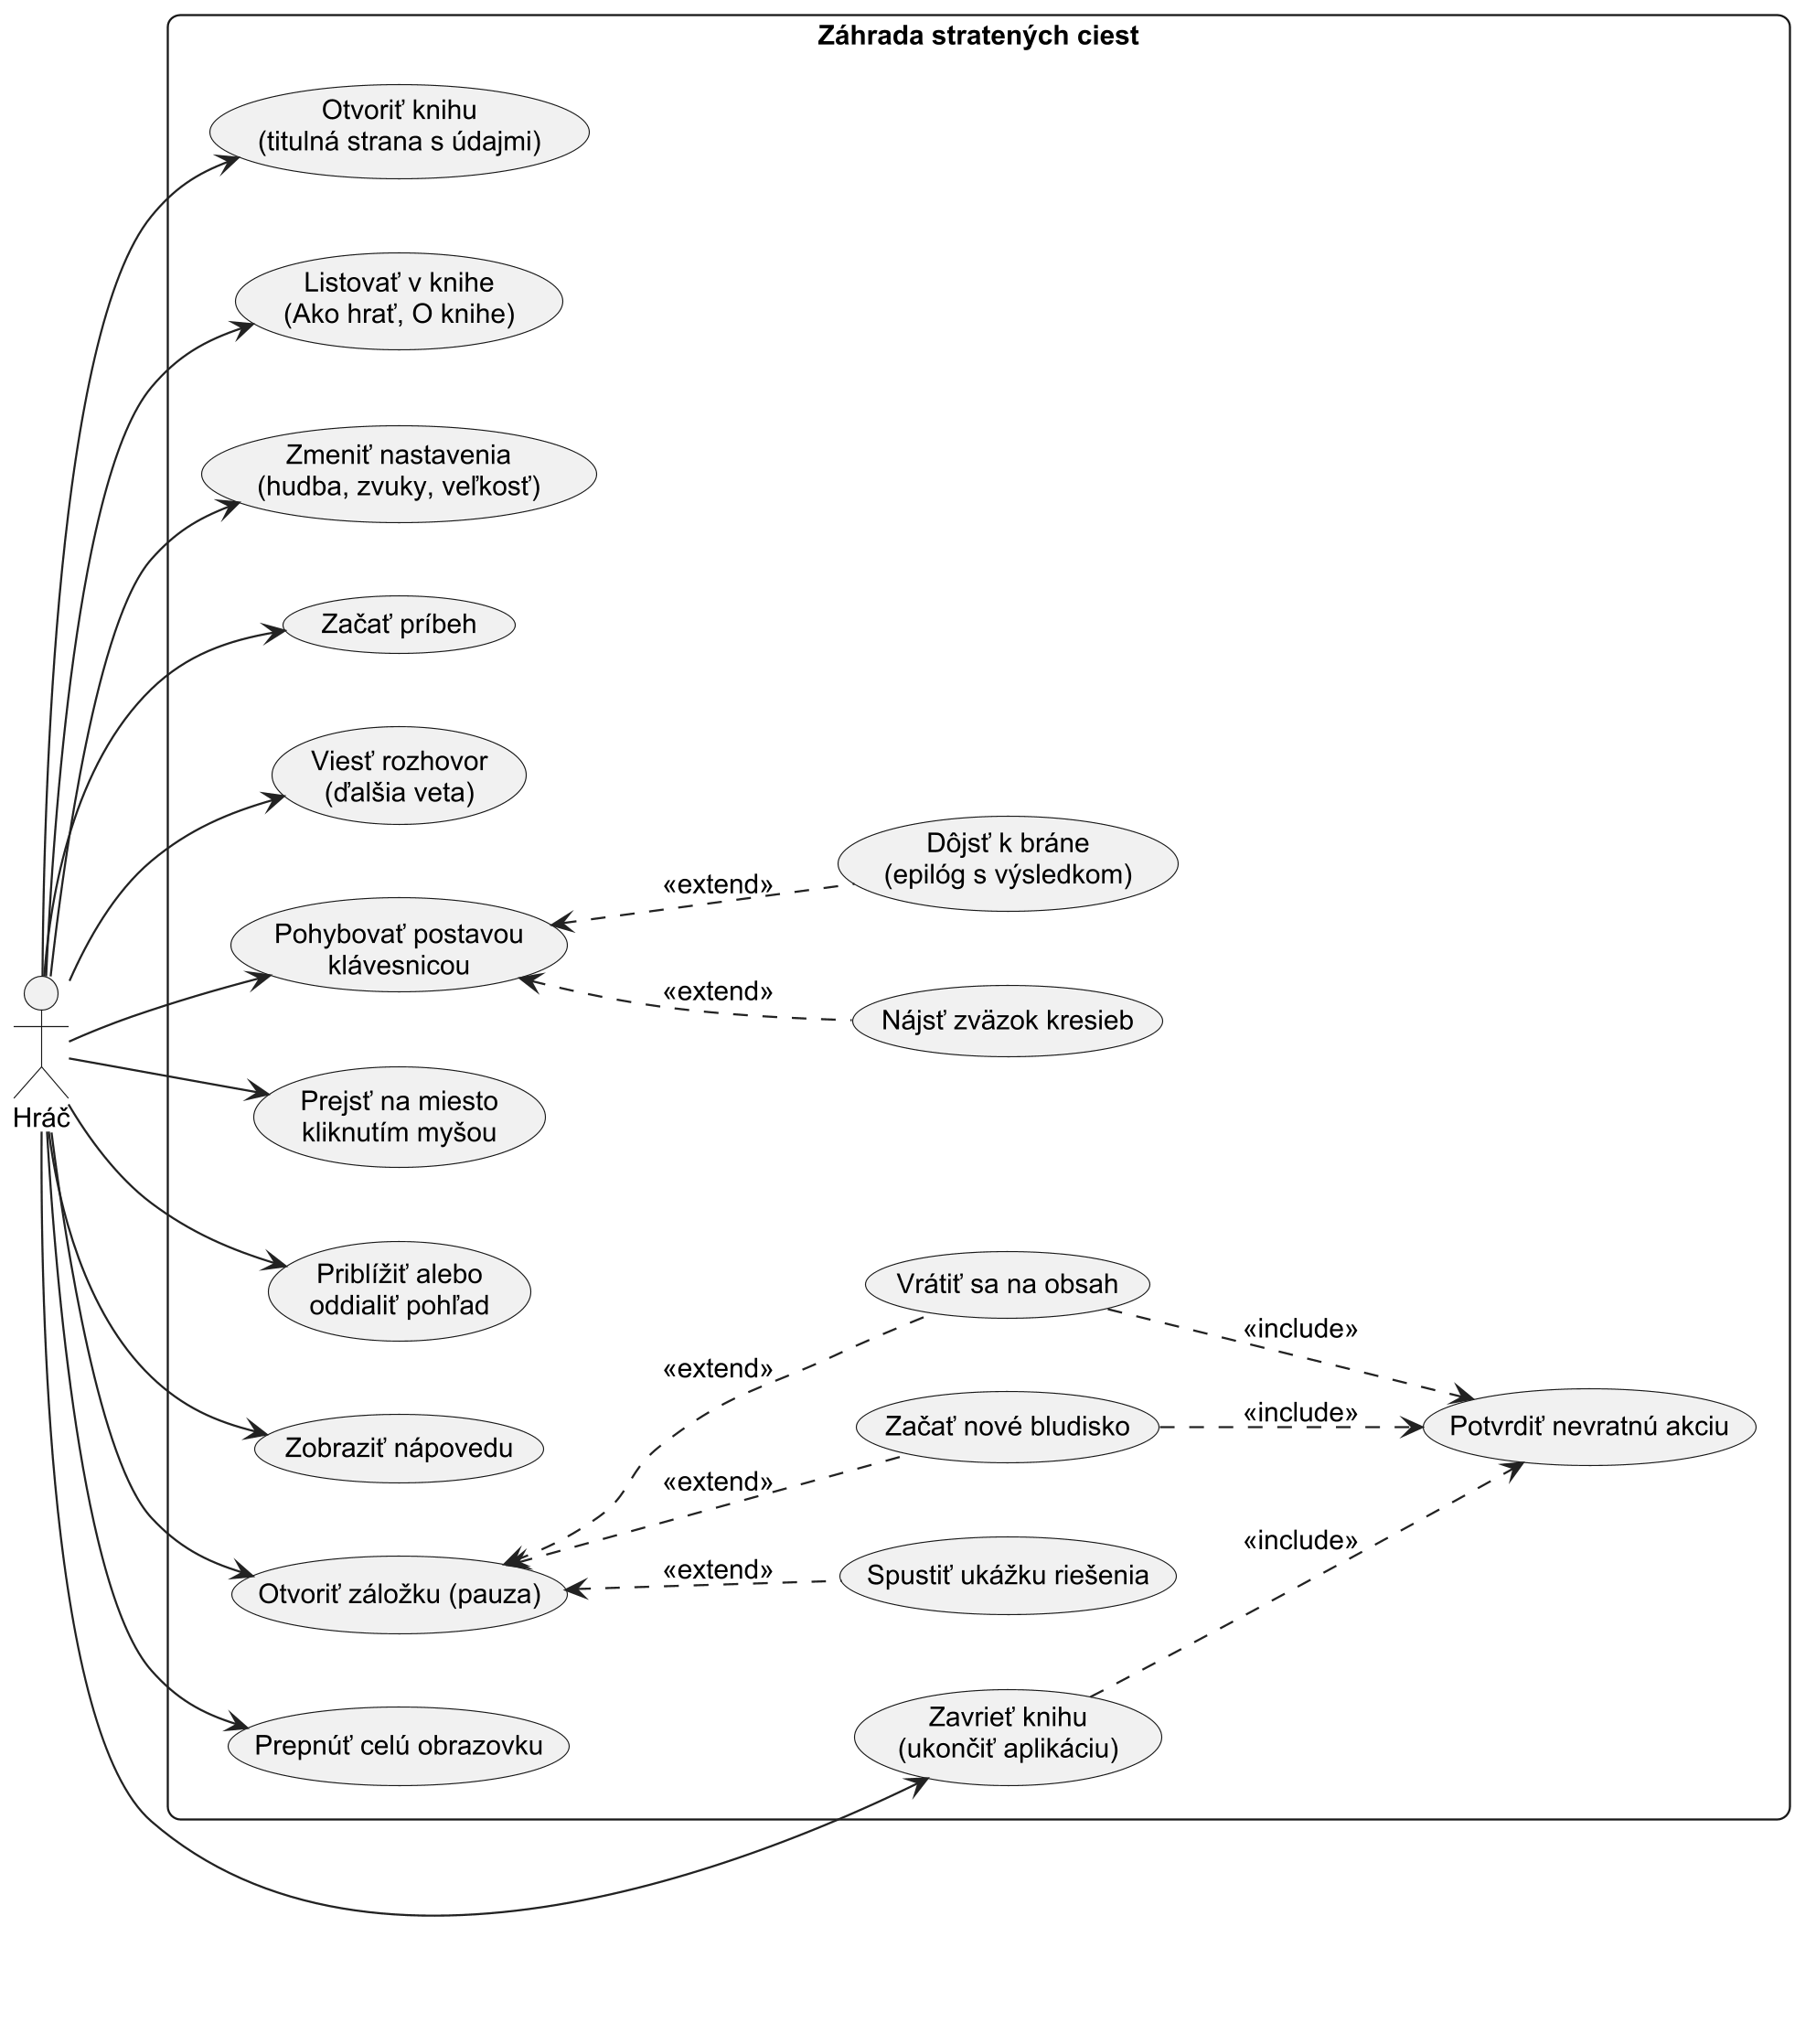
\includegraphics[width=0.78\textwidth]{pouzitie.png}
  \caption{Diagram použitia (use-case)}
\end{figure}

\subsubsection{Izometrická projekcia a súradnicový reťazec}

Svet je pravouhlá mriežka buniek; bunka $(x, y)$ je kocka terénu. Na obrazovku sa zobrazuje
rovnobežným (axonometrickým) premietaním~\cite[kap.~5]{Sobota2024}, v~ktorom os $x$ mriežky
smeruje vpravo dole a os $y$ vľavo dole. Stred hornej steny kocky má svetové súradnice
\begin{equation}
  x_w = (x - y)\, a, \qquad y_w = (x + y)\, b,
  \label{eq:iso}
\end{equation}
kde $a = 80$ px je polovica šírky a $b = 44$ px polovica výšky kosoštvorca hornej steny
(pomer $a : b \approx 2 : 1$ zodpovedá dimetrickej projekcii používanej v~hrách).
Inverzná transformácia (bunka pod kurzorom myši) vznikne riešením sústavy~\eqref{eq:iso}
a zaokrúhlením na najbližšiu bunku:
\begin{equation}
  u = \frac{x_w}{a},\quad v = \frac{y_w}{b},\qquad
  x = \operatorname{round}\!\left(\frac{v + u}{2}\right),\quad
  y = \operatorname{round}\!\left(\frac{v - u}{2}\right).
\end{equation}
Celý súradnicový reťazec~\cite[kap.~4]{Sobota2024} je: bunka mriežky → svetové súradnice
(rovnica~\ref{eq:iso}) → kamera (posun o~stred záberu $(c_x, c_y)$ a zmena mierky
o~priblíženie $z$) → pixely plátna:
\begin{equation}
  x_p = (x_w - c_x)\,z + \tfrac{W}{2}, \qquad y_p = (y_w - c_y)\,z + \tfrac{H}{2}.
  \label{eq:kamera}
\end{equation}
Plátno má rozmer okna v~skutočných pixeloch displeja (násobok \subor{devicePixelRatio}),
preto je kresba ostrá aj pri zväčšení vo Windows a na monitoroch 2560 × 1440.

\subsubsection{Riešenie viditeľnosti – maliarov algoritmus}

Kresby sa navzájom prekrývajú (strom za domom, postava za plotom). Viditeľnosť sa rieši
maliarovým algoritmom~\cite[kap.~7]{Sobota2024}: objekty sa kreslia od najvzdialenejších
k~najbližším. V~izometrickom pohľade je vzdialenosť od pozorovateľa daná diagonálou $x + y$,
v~rámci jednej bunky ešte vrstvou (terén, detail, stopa, predmet, postava):
\begin{equation}
  \text{hĺbka} = 10\,(x + y) + \text{vrstva}, \qquad \text{vrstva} \in \{0, 1, 2, 3, 4\}.
\end{equation}
Phaser pred vykreslením zoradí objekty podľa hĺbky. Postavy a zvieratá sa pohybujú plynulo,
ich diagonála sa preto vypočíta z~polohy päty $y_w$ (funkcia \subor{depthAt}):
\begin{equation}
  \text{hĺbka} = 10\,\frac{y_w}{b} + \text{vrstva}.
\end{equation}
Živé ploty sú vysoké a v~úzkej chodbe by postavu od pása dole zakryli. Počas hry preto ploty
na troch bunkách tesne pred postavou (bližšie ku kamere: $(x{+}1, y)$, $(x, y{+}1)$,
$(x{+}1, y{+}1)$) plynulo priesvitnú na 38 \% (časová konštanta 160 ms) a po odchode postavy
sa vrátia (\subor{seeThroughHedges}) – postavu aj chodník je vidno celé.
Diagonála je neceločíselná: kým postava prechádza z~diagonály $d$ na $d + 1$, živý plot na
diagonále $d + 1$ vedľa nej ju ešte zakrýva a postava ho „predbehne“ až tesne pred cieľom,
keď sa už neprekrývajú. Postava tak nikdy nevystúpi nad plot pred sebou. Výnimkou je paluba
mosta a móla, ktorá je nad terénom – tam sa diagonála zaokrúhli nahor, aby dosky nezakryli
nohy chodca. Terén (dlaždice, chodníky) je v~samostatnej vrstve kreslenej pred všetkými
predmetmi, preto postava nikdy nie je pod dlažbou. Nad ním leží malá vrstva povrchu – vlnky,
kruhy na vode a stopy, ktoré stále vznikajú a zanikajú; vo vrstve terénu s~tisíckami dlaždíc
by každé pridanie znamenalo nové zoradenie celej vrstvy podľa hĺbky (merané až 30 ms snímky
v~daždi).

\subsubsection{Papier a farby}

Svet je čierny atrament na bielom podklade. Po nakreslení sa naň položí jedna opakovaná textúra
papiera v~režime násobenia (\subor{BlendModes.MULTIPLY}); pre každú zložku RGB s~hodnotami
v~intervale $\langle 0, 1\rangle$ platí
\begin{equation}
  C = C_{\text{kresba}} \cdot C_{\text{papier}},
\end{equation}
takže biela plocha kresby prevezme farbu a zrno papiera a čierna čiara zostane čierna.
Textúra papiera je ukotvená k~súradniciam sveta, pri pohybe kamery sa teda neposúva voči kresbe.
Vzdialené časti sveta sa zosvetľujú (vzdušná perspektíva) farebným odtieňom v~režime
\emph{screen} so šedou $T$, ktorá rastie lineárne so vzdialenosťou za bludiskom
($T = 0{,}18$ až $0{,}6$):
\begin{equation}
  C = 1 - (1 - C_{\text{kresba}})(1 - T).
\end{equation}
Rovnaký odtieň zosvetľuje tmavú kresbu vody. Objekty, ktoré sa objavujú alebo miznú (kvapky,
mláky, bubliny, stopy), používajú alfa miešanie~\cite[kap.~1]{Sobota2024}
$C = \alpha\, C_s + (1 - \alpha)\, C_d$. Pri okrajoch obrazovky a pod poznámkami v~rohoch sa
kresba stráca v~čistom papieri: medzi kresbu a papier sa vloží biela vrstva s~radiálnym
prechodom priehľadnosti.

Kresba sveta na strane knihy vzniká mimo obrazovky (kapitola~\ref{sec:lod}) a má byť
atramentom na papieri strany. Preto sa biela zmení na priehľadnosť: pre pixel s~najmenšou
zložkou $w = \min(R, G, B)$ (podiel bielej) je priehľadnosť a farba atramentu
\begin{equation}
  \alpha = 1 - w, \qquad C' = \frac{C - w}{1 - w},
\end{equation}
čo na bielom podklade dáva presne pôvodnú farbu ($\alpha C' + (1 - \alpha) = C$) a na papieri
strany prakticky to isté ako násobenie – bez nákladného miešania vrstiev v~každom snímku.

\subsubsection{Úroveň detailov a orezanie}\label{sec:lod}

Svet má okolo 7\,000 kresieb. Počas hry je v~zábere kamery len ich zlomok, preto sa pred
vykreslením nastaví viditeľnosť podľa obdĺžnika záberu (orezanie, \subor{cull}); kotvou kresby je
jej päta. Rezerva okolo záberu zodpovedá najväčšiemu presahu kresby od päty, zmeranému
v~atlase: dlaždice terénu siahajú najviac 65 px nad pätu, 117 px pod ňu a 124 px nabok
(rezerva 80, 130 a 130 px), stromy a veže až 537 px nad pätu (rezerva 600 px zospodu záberu).
Samostatná, tesnejšia rezerva pre terén ušetrí asi tretinu kreslených dlaždíc. Prechod všetkými
kresbami trval vyše 3 ms, preto sa rozdelí na tri snímky – každý snímok sa preverí tretina
kresieb (každá tretia v~zozname) a čas klesol na približne 1 ms; keď sa svet práve ukáže
(prebudenie, koniec obrazu z~výšky), preveria sa všetky naraz. Rezerva je oveľa väčšia, ako
sa kamera za tri snímky posunie, takže oneskorenie nie je vidno. Z~veľkej výšky (pri lete
kamery) by bolo vidno celý svet naraz, preto sa vtedy nekreslia jednotlivé kresby, ale jediný obraz
celého ostrova nakreslený vopred mimo obrazovky do textúry \subor{DynamicTexture}
(\subor{drawFarView}). Podľa pomeru $r$ priblíženia kamery k~priblíženiu celého ostrova sa obraz
a živý svet prelínajú:
\begin{equation}
  \alpha_{\text{obraz}} = 1 - \operatorname{smoothstep}(1{,}3;\; 1{,}7;\; r),
\end{equation}
kde $\operatorname{smoothstep}(a, b, x) = s^2 (3 - 2s)$, $s = \operatorname{clamp}\bigl((x - a)/(b - a)\bigr)$.
Do rovnakej textúry (v~polovičnom rozlíšení) sa kreslí aj kresba do knihy; pixely sa z~nej
prečítajú funkciou \subor{readPixels}~\cite{MdnReadPixels} až o~dva snímky neskôr, keď ich
grafická karta dokreslila, aby čítanie nečakalo na grafickú kartu.

\subsubsection{Kamera počas hry}

Kamera počas hry sleduje cieľ plynulo – priblíženie aj stred sa každý snímok priblížia k~cieľu
exponenciálne s~časovou konštantou $\tau$ ($\tau_z = 160$ ms, $\tau_c = 260$ ms):
\begin{equation}
  \ln z_{k+1} = \ln z_k + (\ln z^* - \ln z_k)\bigl(1 - e^{-\Delta t / \tau_z}\bigr),
\end{equation}
priblíženie sa teda mení v~logaritmickej mierke (rovnaký zárez kolieska je vždy rovnako veľký
krok, $z^* = z_{\text{hra}} \cdot 1{,}15^{-n}$ pre $n$ zárezov). Cieľový stred je zmes stredu
bludiska a polohy postavy podľa priblíženia; pri pohľade na celé bludisko kamera stojí, po
priblížení sleduje postavu. Záber nikdy nevyjde za okraj sveta (obdĺžnik vpísaný do kosoštvorca
sveta).

\subsubsection{Let kamery medzi knihou a svetom}

Najvýraznejší prechod aplikácie je jeden nepretržitý záber z~knihy na stole do sveta (a späť).
Kresba na strane je snímka sveta pri pohľade na celý ostrov, preto kniha aj svet tvoria
jednu „mapu“. Ak $C$ je obdĺžnik kresby na strane, $z_0$ priblíženie sveta, ktoré mu zodpovedá,
$P$ cieľový bod sveta (napr. stred medzi hráčom a záhradníkom) a $F$ poloha bodu $P$ na kresbe,
potom pri priebehu letu $u \in \langle 0, 1 \rangle$
\begin{equation}
  s(u) = e^{L u}, \quad L = \ln\frac{z_1}{z_0}, \qquad
  \mathbf{q}(u) = \mathbf{F} + (\mathbf{S} - \mathbf{F})\,u, \qquad z(u) = z_0\, s(u),
\end{equation}
kde $s$ je zväčšenie knihy, $\mathbf{q}$ poloha bodu $P$ na obrazovke ($\mathbf{S}$ je stred
obrazovky) a $z$ priblíženie kamery sveta. Mierka sa mení geometricky – rovnaký úsek letu
priblíži vždy rovnakým pomerom, čo oko vníma ako rovnomerný let~\cite{VanWijk2003} –,
a cieľový bod sa po obrazovke presúva rovnomerne do stredu, takže kamera neuhýba do strán.
Kamera knihy je transformácia CSS \subor{translate(q − F) scale(s)} s~počiatkom v~bode $F$;
kamera sveta má podľa~\eqref{eq:kamera} stred $\mathbf{c} = \mathbf{P} - (\mathbf{q} - \mathbf{S})\,r / z$
($r$ je počet pixelov plátna na pixel CSS). Čas letu $t$ sa pretvorí krivkou
$u = 6t^5 - 15t^4 + 10t^3$ s~nulovou rýchlosťou aj zrýchlením na začiatku a na konci.

Kniha sa so svetom prelína od chvíle, keď má kresba polovicu veľkosti, pri ktorej zakryje celú
obrazovku ($u_\text{clear} = u_\text{solid} - \ln 2 / L$), do chvíle, keď ju zakryje
($u_\text{solid}$, nájde sa numericky). Hra sa prebudí o~kúsok skôr, pod ešte nepriehľadnou
knihou. Let knihy je animácia Web Animations so 120 snímkami, ktorú prehliadač skladá na
grafickej karte; kamera sveta sa nastaví tesne pred vykreslením každého snímku hry (udalosť
\subor{prerender}) z~času toho istého snímku, meraného od začiatku tej istej animácie – kresba
a svet sa preto v~každom snímku presne kryjú. Vývojový diagram je na obrázku~\ref{fig:let}.

\subsubsection{Kniha: doska, listy a písanie}

\paragraph{Doska} sa otáča okolo chrbta (\subor{rotateY} od $0°$ po $-180°$) jedným plynulým
pohybom ruky (časová funkcia \subor{cubic-bezier(0.6, 0, 0.3, 1)}, 1,5 s); kniha sa pritom
posunie do stredu stola. Zvuk otvorenia je naplánovaný na hodinách zvukového systému na
okamih, keď doska dosadne (80 \% trvania). Rub dosky je kópia ľavej strany knihy, ktorá sa
po dosadnutí nenápadne prelínaním vymení za skutočnú stranu. Tieň knihy na stole je vopred
rozostrený obrázok natiahnutý cez \subor{border-image}, nie filter \subor{drop-shadow}, ktorý
by prehliadač musel rozostrovať v~každom snímku.

\paragraph{List} sa otáča ako ohýbajúci sa papier. Je zložený z~$N = 10$ zvislých pásikov,
každý je vnorený v~predchádzajúcom a otáča sa okolo jeho okraja (prvý okolo krúžkov väzby).
Pásik $i$ so vzdialenosťou od chrbta $s_i = (i + \tfrac12)/N$ má v~čase $t$ uhol
\begin{equation}
  \theta_i(t) = \pi\, e\!\left(\frac{t - a_i}{1 - 2a_i}\right), \qquad a_i = \lambda (1 - s_i),
  \qquad e(x) = x - k\,\frac{\sin(2\pi x)}{2\pi}, \; x \in \langle 0, 1 \rangle,
\end{equation}
($\lambda = 0{,}22$, $k = 0{,}6$ – list sa pohne hneď po kliknutí a dopadne s~malou
rýchlosťou), takže okraj listu sa zdvihne prvý a dopadne posledný a list sa pritom prehne;
vnorený pásik sa otáča o~rozdiel $\theta_i - \theta_{i-1}$. Uhly sa vopred vypočítajú do
40 kľúčových snímok a prehrajú ako animácie Web Animations iba s~transformáciami
a priehľadnosťou, ktoré skladá grafická karta – list sa otáča plynulo aj na pomalšom
procesore. Kópie strán na liste ukazujú stranu v~konečnom stave bez animácií a strana, ktorá
už v~knihe leží, sa nevkladá znova, aby sa jej animácie (vpíjanie kresby) neopakovali. Rozmery
listu sa počítajú presne (bez zaokrúhlenia na pixely), takže dopadnutý list leží presne na
skutočnej strane; tá sa vloží pod list a list sa do nej krátko prelínaním rozplynie.
Pri preskočení viacerých dvojstrán (napr. z~obsahu na stranu O~knihe) sa otočí toľko listov,
koľko dvojstrán sa preskočí (najviac štyri), rýchlo za sebou s~odstupom 120 ms – každý list
nesie svoje strany a ich poradie nad sebou sa v~polovici otočenia (pri chrbte) vymení. Každý pásik má líce
(výrez otáčanej strany) a rub (výrez strany na druhej strane listu) so skrytou zadnou stenou
(\subor{backface-visibility}). Naklonený papier tmavne úmerne $\sin\theta_i$ a zdvihnutý list
vrhá na stranu pod sebou tieň. Papier každej strany je presný výrez z~obrázka otvorenej knihy
bez krúžkov, preto strany splývajú s~knihou pod nimi. Krúžky sa kreslia nad stranami aj
s~tieňmi a otvormi v~papieri z~pôvodného obrázka: priehľadnosť tieňa je o~koľko bol pôvodný
pixel tmavší než papier, $\alpha = 1 - L_{\text{pôvodný}} / L_{\text{papier}}$, takže pokojná
kniha vyzerá presne ako pôvodný obrázok.

\paragraph{Písanie.} Slová textu sú na strane od začiatku na svojom mieste, len neviditeľné;
každé sa vynorí animáciou priehľadnosti s~oneskorením, takže sa text pri písaní neposúva.
Oneskorenie slova je čas, keď ho rozprávač vysloví (časy slov z~nahrávky, pozri ďalej odsek
Hlasy); odsek nasleduje 450 ms po dočítaní predchádzajúceho. Bez hlasu sa slová píšu po
$\Delta = 70 + 26\cdot\text{počet písmen}$ ms. Ceruzka škrabe pri každom slove a medzi slovami
sa takmer zdvihne. Počas písania
znie súvislé škrípanie ceruzky, ktoré po dopísaní dozneje. Slučku ceruzky hrá priamo Web Audio
(zdroj \subor{AudioBufferSource} s~opakovaním úseku nahrávky a zosilňovač \subor{GainNode}),
lebo herná slučka knižnice Phaser počas scén v~knihe spí a jej zvuky by sa po prvom opakovaní
zastavili. Hlasitosť sa mení plynulo (\subor{setTargetAtTime}, časová konštanta 40 ms), preto
zmeny tempa písania nepraskajú.

\paragraph{Hlasy.} Všetky vety, ktoré zaznejú, sú v~scenári \subor{story.js}. Nástroj
\subor{hlasy.py} každú nahovorí cez službu ElevenLabs~\cite{ElevenLabs} modelom
\subor{eleven\_v4}, ktorý hovorí s~prirodzenou intonáciou aj po slovensky (jazyk vety
\subor{sk}): rozprávač má hlas George (vrúcny rozprávač), babka Lily (pomalšie tempo, 0,9),
záhradník Bill (starší muž) a myšlienky postavy Jessica (mladý hlas). Výslovnosť sa overila
automatickým prepisom reči (Whisper): 35 z~39 viet rozpoznal ako slovenčinu (ostatné ako
blízku češtinu); rozdiely prepisu sú väčšinou pravopisné (napr. ä vyslovené ako e). Služba
spolu so zvukom vráti čas začiatku každého znaku vety; čas slova (delenie medzerami ako
v~hre) je čas jeho prvého znaku. Nástroj ho uloží s~dĺžkou nahrávky do
\subor{audio/hlas/hlasy.json}. Nahrávky majú zjednotenú hlasitosť (EBU R128, $-17$ LUFS).

Hra hľadá nahrávku podľa textu vety (\subor{SoundDirector.voiceOf}), takže scenár a hlasy
spája len text. Reč hrá priamo Web Audio (\subor{speak}) ako ceruzka – znie aj v~knihe, kde
herná slučka spí. Kým niekto hovorí, hudba plynulo stíchne na 35 \% a zvuky prostredia na 60 \%
(exponenciálne, časová konštanta 350 ms). Bublina rozhovoru píše slová v~časoch ich začiatku
(\subor{writeLine}) a zavrie sa po $\max(t_{\text{reč}},\ 55\,\text{ms} \cdot n) + 900$ ms,
kde $n$ je počet znakov – vetu stihne povedať aj prečítať pomalší čitateľ. Titulky so spomienkou
zostanú $\max(2600 + 55 n,\ t_{\text{reč}} + 900)$ ms. Pri záložke, novom svete či začiatku
záverečnej scény reč doznie (\subor{hush}).

\subsubsection{Animácia sveta}

Všetky pohyby sú interpolácie medzi dvoma stavmi s~časovou funkciou (easing) knižnice Phaser.
Krok postavy z~bunky $P_0$ do $P_1$ trvá 240 ms; pre $t \in \langle 0, 1\rangle$
\begin{equation}
  P(t) = (1 - t)\,P_0 + t\,P_1 - \bigl(0,\; h\,|\sin(2\pi t)|\bigr), \qquad h = 3 \text{ px},
\end{equation}
teda dva kroky na bunku; postava sa pritom kolíše o~$\pm 2°$ a v~polovici a na konci kroku
na zemi ostane stopa (sploštená v~pomere $b/a$ do roviny terénu); zvuk kroku zaznie raz
na bunku. Chodci kráčajú
rovnako, ich trasu po cestách dediny hľadá A*; každý ide inou rýchlosťou (dospelí 0,8 až
1,15-násobok, deti sú menšie – 78 \% – a ponáhľajú sa). Okrem domácich a pasúcich sa zvierat
skáču po námestí a dvore vrabce, po poliach vrany a lesom sa zakráda líška; pri domoch stoja
bicykel, pumpa, vrecia či hniezdo, v~lese a v~parku ležia kamene, mach, lístie a haluzky. Zajac a žaba skáču: k~lineárnej interpolácii
polohy sa pripočíta $h\,|\sin(\pi k t)|$, kde $k$ je počet skokov. Zviera sa presunie len na
bunku, kam vedie voľná priama cesta (kontrola každej štvrtiny bunky), a drží si odstup od
ostatných zvierat. Stromy a trstina sa kolíšu okolo päty o~$\pm 1{,}6°$ so sínusovým priebehom,
ktorého fáza závisí od polohy $x$ – poryv vetra tak prechádza krajinou.

Voda fontány, dážď a semienka vo vetre sú systémy častíc. Kvapka fontány vyletí rýchlosťou
190 až 240 px/s pod uhlom $205°$ až $240°$ (resp. $300°$ až $335°$) a padá so zrýchlením
$g = 560$ px/s$^2$:
\begin{equation}
  x(t) = x_0 + v_{0x} t, \qquad y(t) = y_0 + v_{0y} t + \tfrac{1}{2} g t^2.
\end{equation}
Kvapky dažďa padajú pod uhlom $108°$ rýchlosťou približne 1\,500 px/s a každá zanikne v~náhodnej
výške obrazovky. Počasie kreslí samostatná scéna \subor{SkyScene} s~vlastnou kamerou, preto
kvapky nemenia veľkosť pri priblížení kamery sveta. Na rieke vznikajú vlnky, ktoré sa posúvajú
s~prúdom, v~daždi a pri fontáne kruhy na vode.

\paragraph{Začiatok a koniec bludiska.} Po rozhovore so záhradníkom hráč vojde oblúkom do
bludiska a kamera sa zároveň vznesie nad celé bludisko (chôdza a let kamery bežia súčasne),
filmové pásy pritom odídu. Na konci prejde hráč bránou k~babke, kým ich kamera berie do záberu;
po oslave sa hneď začne let kamery späť do knihy. Atrament na papieri (nápoveda, cesta v~cieli,
krúžky ceruzkou) leží vo vlastnej vrstve sveta nad kresbou, ktorá sa pri stavbe nového sveta
zmaže spolu s~ním. Krúžok pod kurzorom sa prepočíta každý snímok (pod kurzorom zostane, aj keď
sa pohne kamera); po kliknutí ostane na cieli väčší krúžok, ktorý sa nakreslí (zväčšenie
s~prekmitom), jemne dýcha ($\pm 6$ \%) a pri príchode postavy sa rozplynie. Keď sú všetky
zväzky pokope, rovnako sa zakrúžkuje výstupná brána.

\paragraph{Myšlienky postavy.} Pri príchode na bunku (\subor{arrive}) postava skontroluje
susedné bunky: ak je v~nich studňa, stĺp alebo záhon zo zákutia (mapa \subor{nooks}), otočí
sa k~nemu, nakloní sa a ukáže sa bublina s~myšlienkou (\subor{think}); každý predmet sa
komentuje raz. Myšlienky má postava aj v~slepej uličke (najviac raz za 20 s), po troch nárazoch
do plota za 5 s a v~miestnosti pred bránou, ak ešte nemá všetky zväzky. Bublina hru nezastavuje, ide s~postavou a po čase
úmernom dĺžke textu vybledne; vety sa striedajú v~náhodnom poradí bez opakovania (\subor{story.js}).

\paragraph{Oslava v~cieli.} Pero nakreslí červeným atramentom prejdenú cestu: hrot sa pohybuje
podľa dĺžky oblúka $\ell(t) = \ell_{\text{celá}} \cdot \tfrac12\bigl(1 - \cos(\pi t)\bigr)$, bod
lomenej čiary sa nájde podľa kumulatívnych dĺžok úsekov. Hlasitosť zvuku pera sleduje rýchlosť
hrotu ($\sqrt{\sin \pi t}$), takže zvuk presne zodpovedá kresleniu. Živé ploty bližšie ako 130 px k~čiare sa pohnú v~okamihu, keď ich
hrot míňa. Na konci cesty z~brány vyletia motýle (let po oblúku – rôzne časové funkcie
pre $x$ a $y$) a vtáky a obrazovkou prefúkne poryv semienok. Rovnaká čiara (s~rovnakým
semienkom chvenia ruky) je potom v~kresbe epilógu.

% -----------------------------------------------------------------------------
\subsection{Popis algoritmov a údajových štruktúr, globálnych premenných}

\subsubsection{Generovanie bludiska}

Bludisko generuje algoritmus Icey's Maze~\cite{RogueBasinMaze} z~knižnice rot.js
(funkcia \subor{createMaze} v~module \subor{maze.js}). Mriežka má nepárny rozmer; bunky s~oboma
nepárnymi súradnicami sú miestnosti, bunky medzi nimi steny alebo prechody. Algoritmus
z~náhodnej vyhĺbenej miestnosti „vŕta“ chodbu do susedných miestností vzdialených o~2,
kým sa nezablokuje, a opakuje to, kým nie sú vyhĺbené všetky miestnosti. Výsledok je
dokonalé bludisko (strom). Program potom otvorí jeden vstup a jednu výstupnú bránu
v~obvodovom plote; cieľom je samotná brána. Malé bludisko má niekedy menej slepých uličiek
než zväzkov (zo 3000 semienok 17~\%); také sa zahodí a skúša sa nasledujúce semienko, kým
bludisko nemá aspoň štyri slepé uličky (tri zväzky a jedno zákutie). V~niektorých slepých uličkách bez zväzku stojí
studňa, stĺp alebo záhon – tieto bunky sa pridajú do množiny \subor{maze.blocked} a funkcia
\subor{isFloor} ich považuje za neprechodné (slepá ulička sa tým len skráti, bludisko zostane
súvislé). Zväzky kresieb ležia v~slepých uličkách: slepé uličky sa zoradia podľa
dĺžky cesty od štartu a pre zväzok $i$ sa vyberie tá, ktorej vzdialenosť je najbližšie
k~$(0{,}3 + 0{,}25\,i)$-násobku najväčšej vzdialenosti – hráč ich tak nachádza postupne.

\begin{figure}[H]
  \centering
  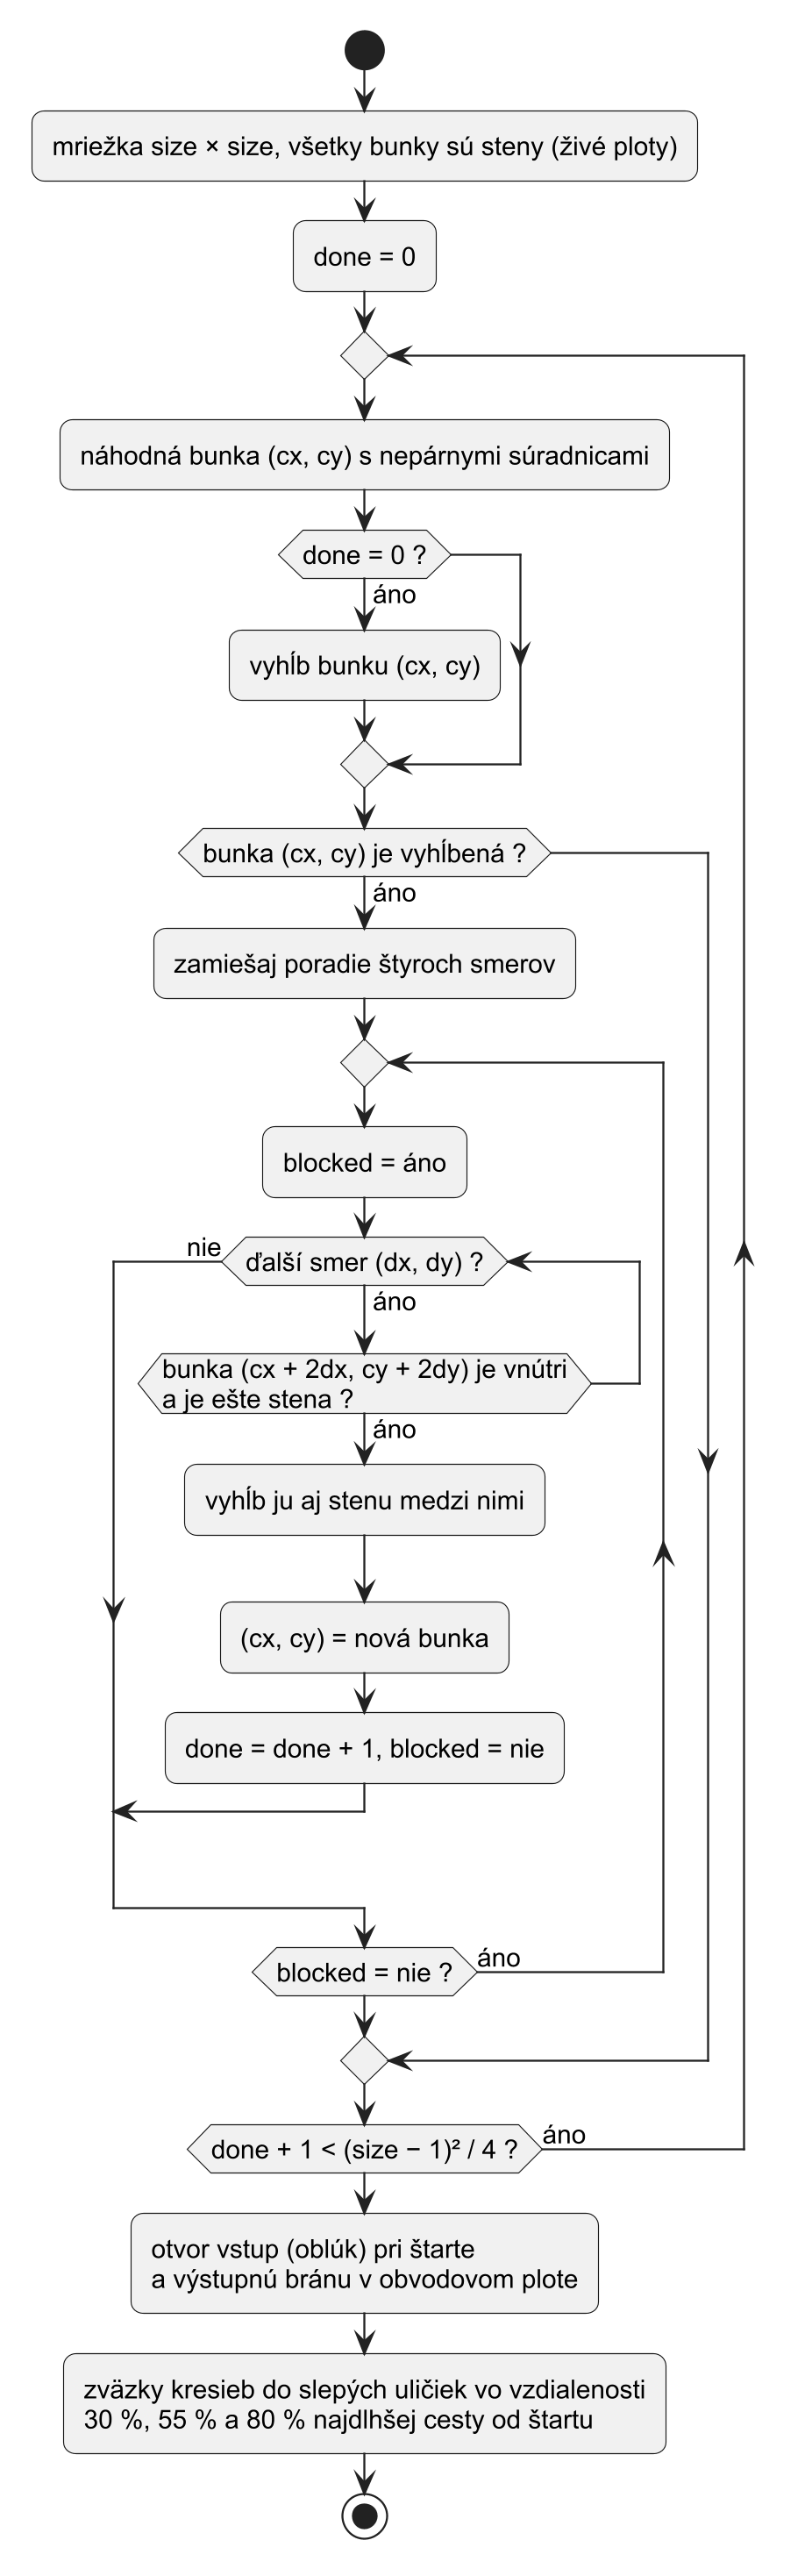
\includegraphics[height=0.6\textheight]{algoritmus-bludisko.png}
  \caption{Vývojový diagram generovania bludiska}
\end{figure}

\subsubsection{Hľadanie najkratšej cesty}

Najkratšiu cestu hľadá algoritmus A*~\cite{Hart1968, RedBlobAStar} (\subor{ROT.Path.AStar},
funkcia \subor{findPath}) so 4-okolím. Cena každého kroku je 1 a heuristika je manhattanovská
vzdialenosť $h = |x - x_s| + |y - y_s|$, ktorá cenu nepreceňuje, preto je nájdená cesta
najkratšia. rot.js hľadá od cieľa k~štartu a cestu potom vracia od štartu. Rovnaký algoritmus
hľadá trasy chodcov po cestách dediny (voľné sú dlažba, cesty a paluby mosta, nie predmety,
voda a lampy; hľadanie je ohraničené okrajom sveta).

\begin{figure}[H]
  \centering
  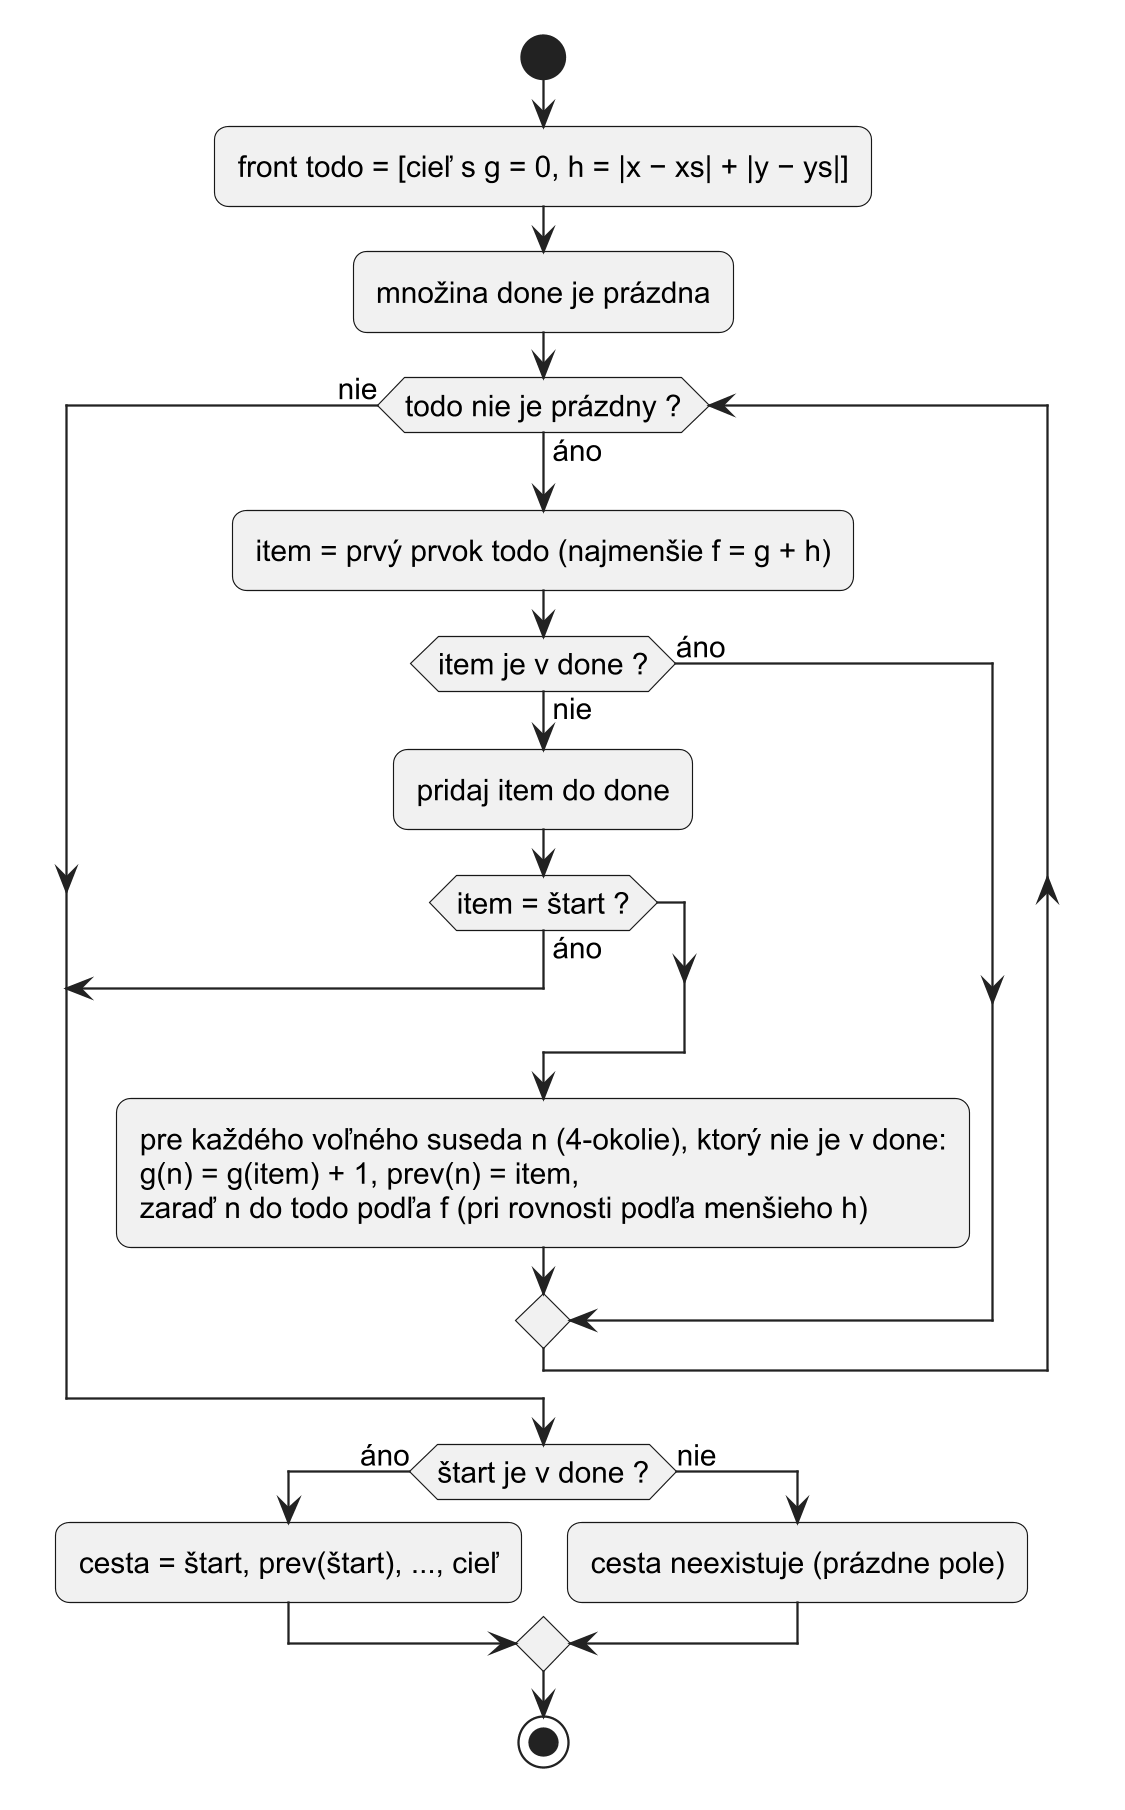
\includegraphics[height=0.5\textheight]{algoritmus-astar.png}
  \caption{Vývojový diagram algoritmu A*}
\end{figure}

\subsubsection{Stavba sveta}

Funkcia \subor{build} vytvorí bludisko a celý svet $68 \times 68$ buniek. Krajina je
rozvrhnutá ako skutočná usadlosť s~bludiskom pri rieke (predlohou je záhrada
Glendurgan~\cite{Glendurgan}): za bludiskom zámok s~nádvorím a fontánou, k~nemu aleja,
vpravo park s~jeleňmi, hospodársky dvor, sad a pastvina, vľavo polia a kostol s~cintorínom,
vpredu ulica s~domami dverami k~ulici, námestie so studňou, rieka s~mostom a mólom, na okraji
les. Kamera sa pozerá zo strany ulice, preto vysoké stavby stoja vzadu. Poloha každej bunky voči
bludisku sa opisuje pásom $r = \max(0, -x, -y, x - (n-1), y - (n-1))$. Os rieky meandruje:
\begin{equation}
  y_r(x) = (n - 1) + 14 + 1{,}2 \sin\frac{x}{9}, \qquad \text{bunka je voda, ak } |y - y_r(x)| \le 1.
\end{equation}

\begin{figure}[H]
  \centering
  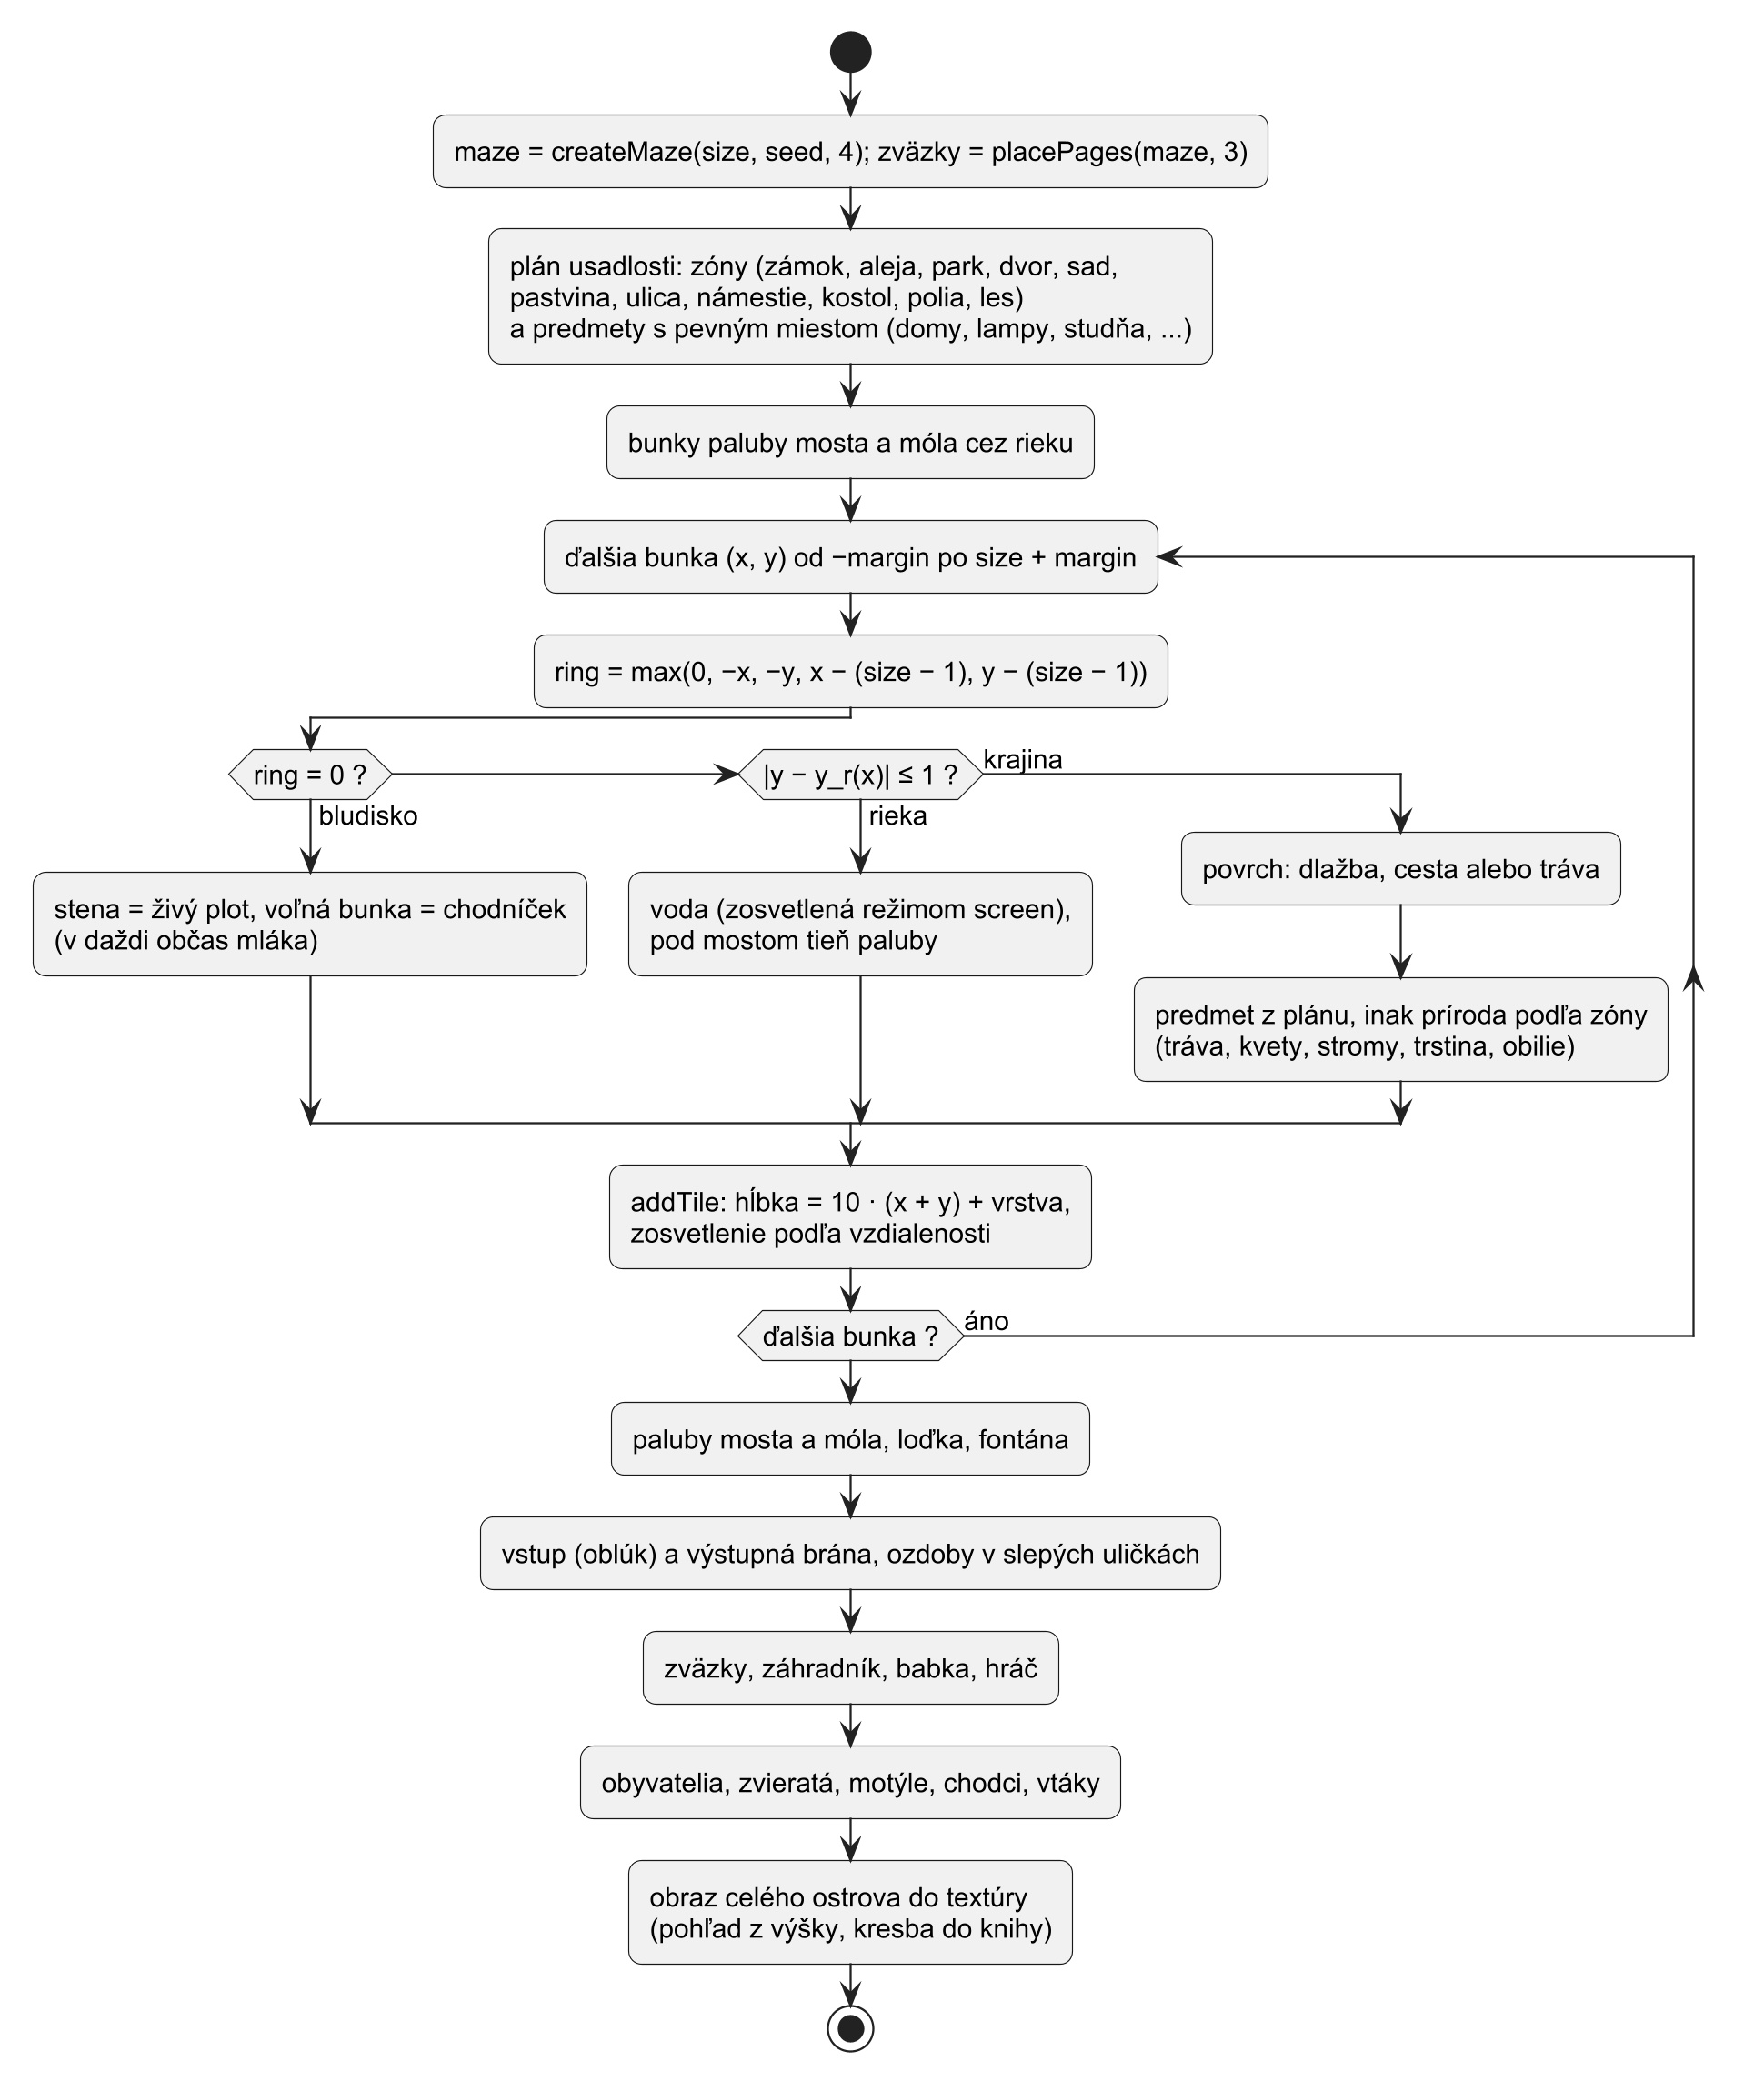
\includegraphics[height=0.62\textheight]{algoritmus-svet.png}
  \caption{Vývojový diagram stavby sveta}
\end{figure}

\subsubsection{Pohyb postavy}

\begin{figure}[H]
  \centering
  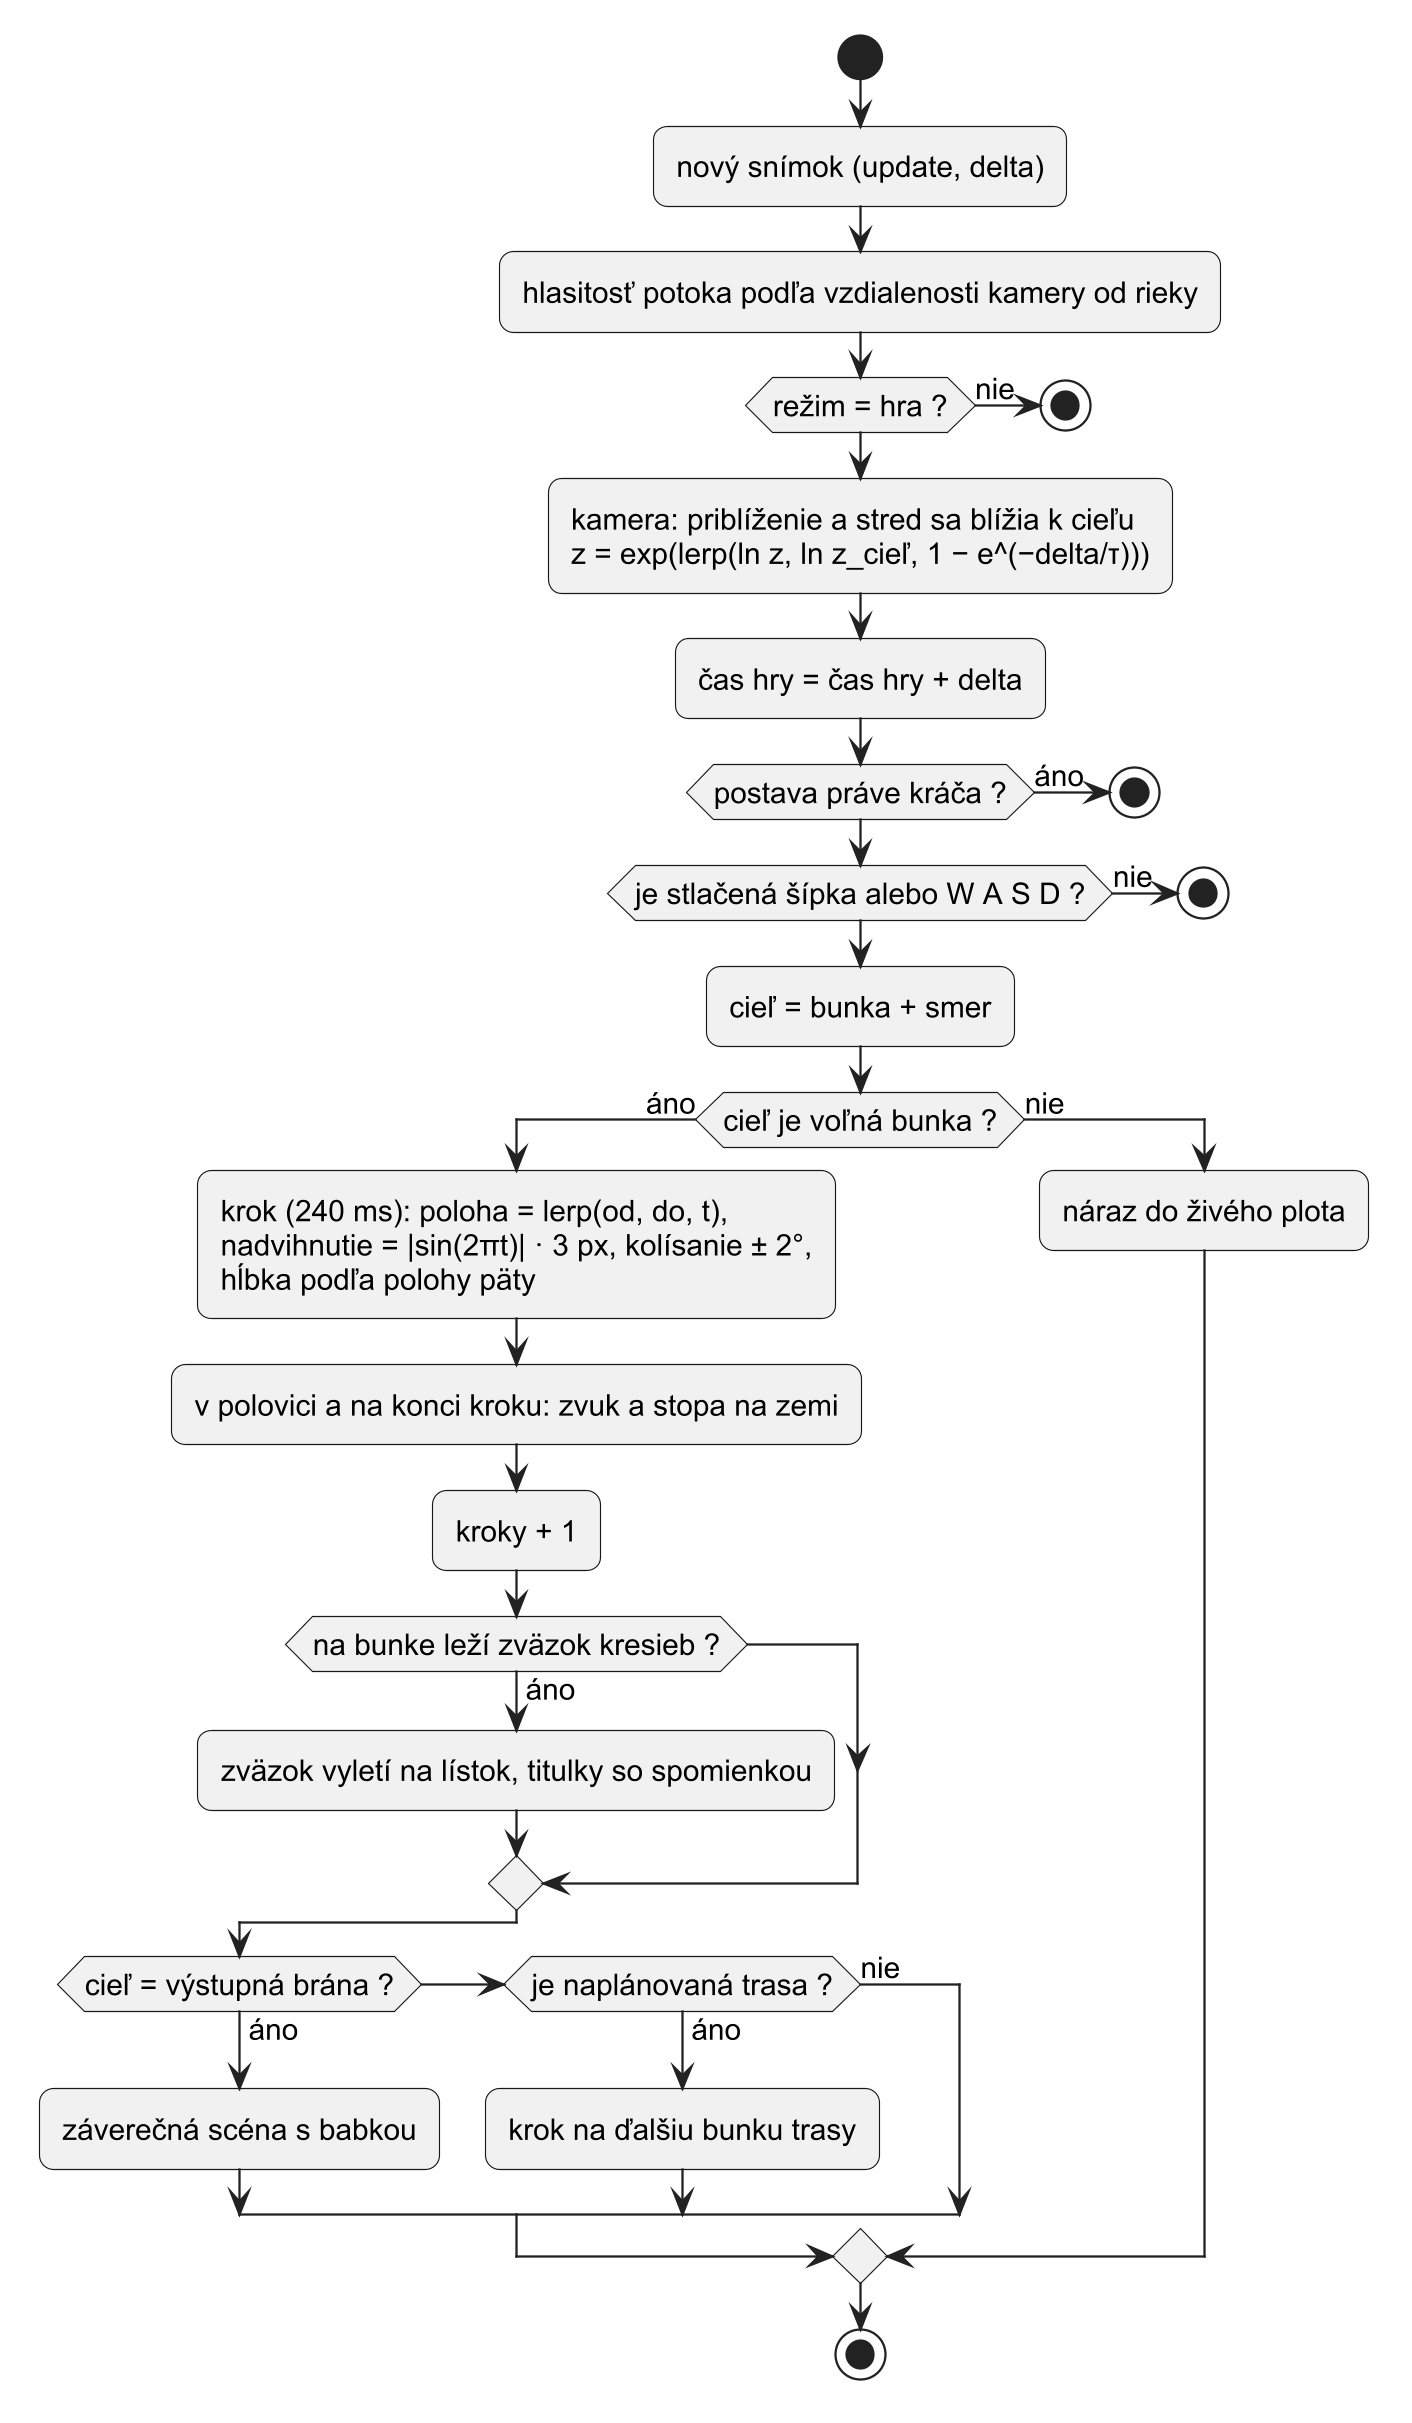
\includegraphics[height=0.62\textheight]{algoritmus-krok.png}
  \caption{Vývojový diagram pohybu postavy v~jednom snímku}
\end{figure}

\subsubsection{Let kamery}

\begin{figure}[H]
  \centering
  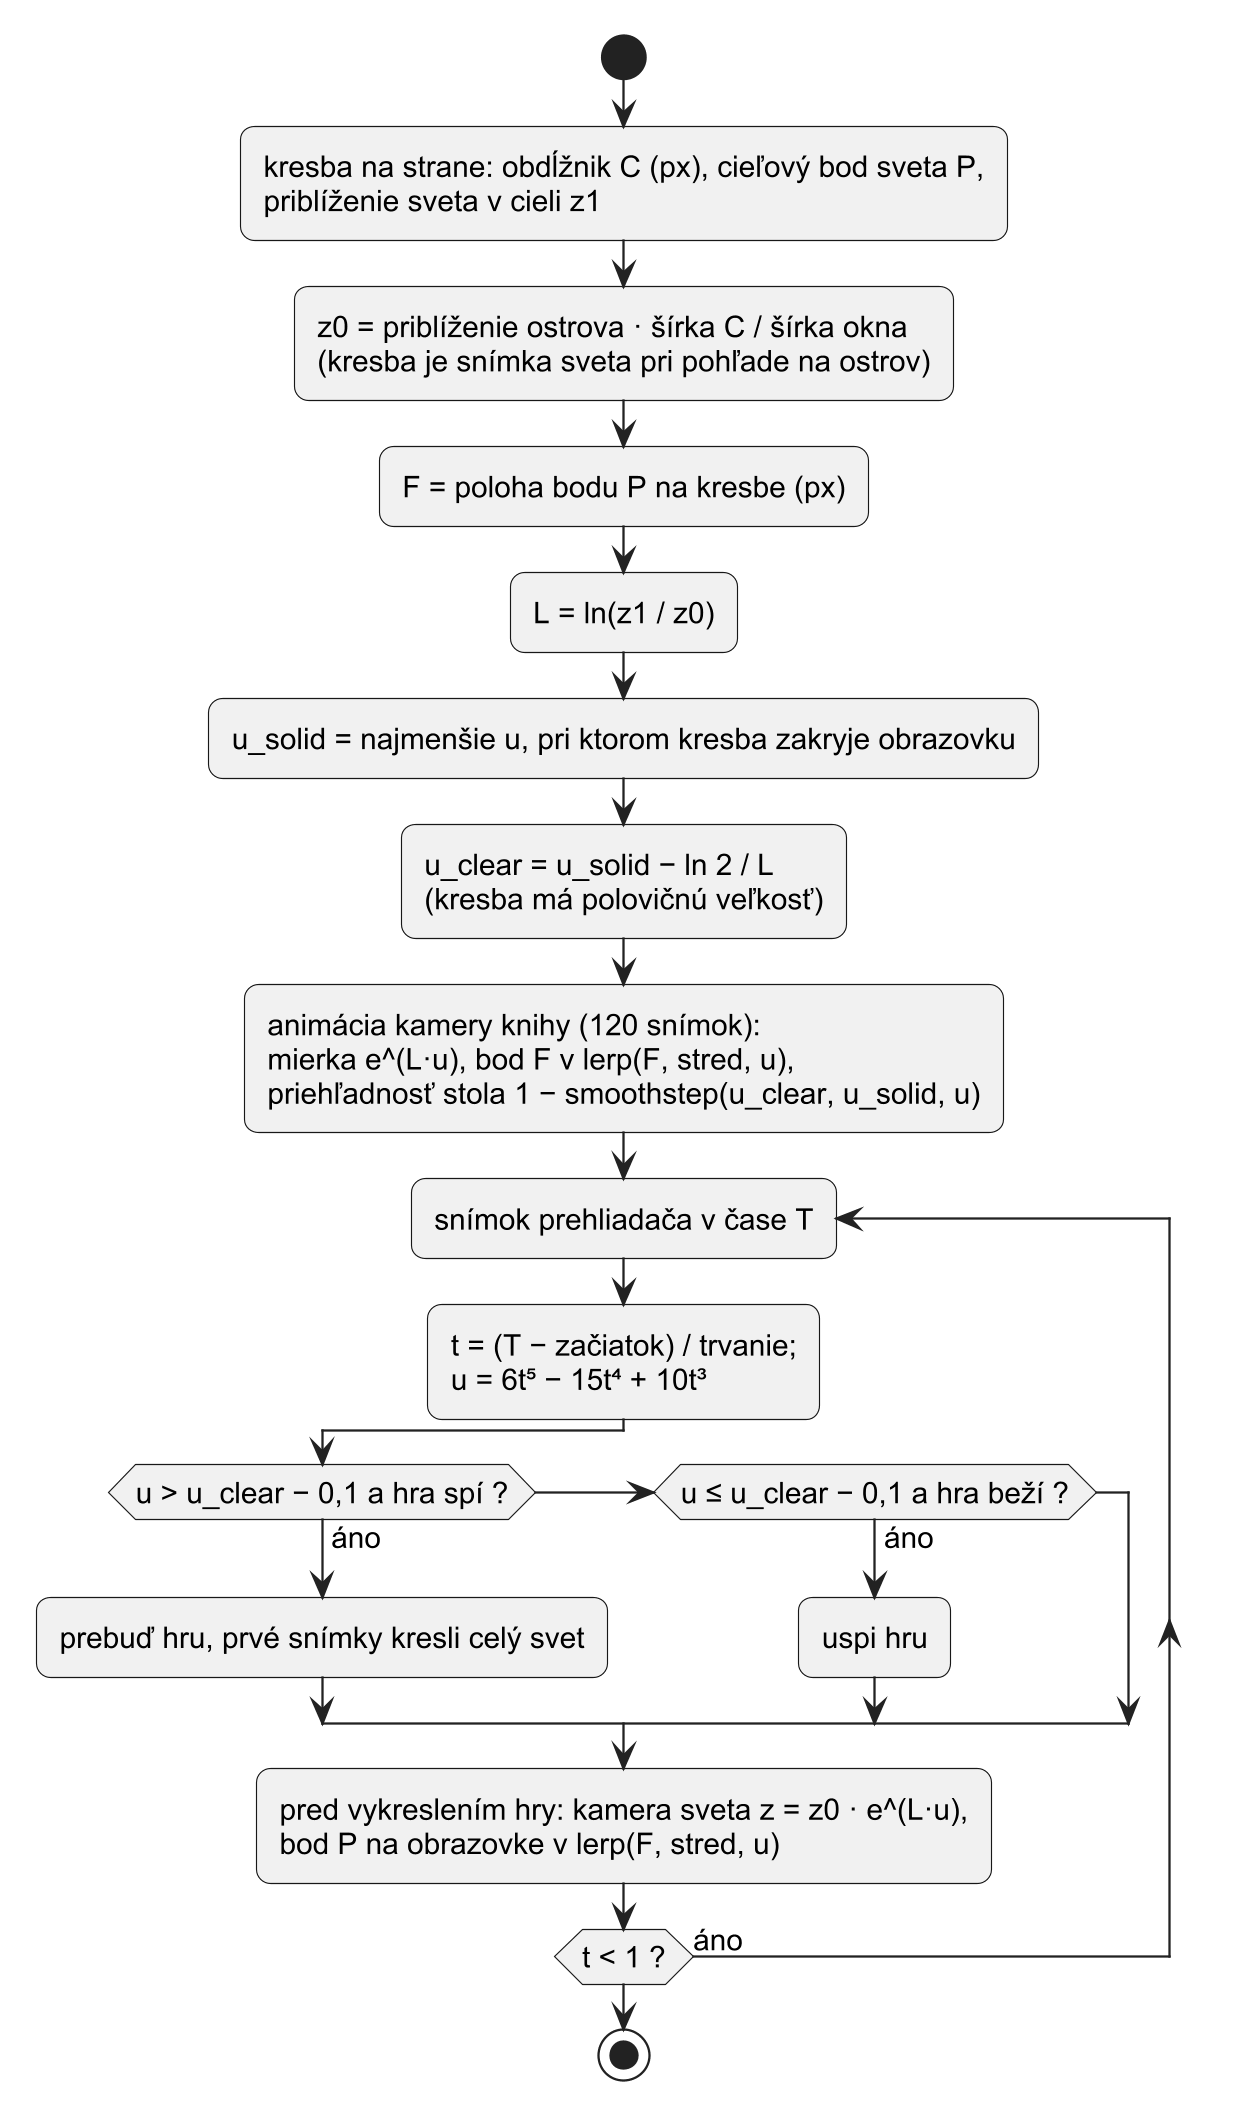
\includegraphics[height=0.66\textheight]{algoritmus-let.png}
  \caption{Vývojový diagram letu kamery medzi knihou a svetom}\label{fig:let}
\end{figure}

\subsubsection{Údajové štruktúry}

\begin{table}[H]
  \centering
  \caption{Hlavné údajové štruktúry}
  \begin{tabularx}{\textwidth}{@{}>{\raggedright}p{0.3\textwidth}X@{}}
    \toprule
    \textbf{Štruktúra} & \textbf{Popis} \\ \midrule
    \subor{maze} (objekt) & \subor{size} – rozmer mriežky, \subor{seed} – semienko, \subor{walls[y][x]} –
      dvojrozmerné pole (true = stena), \subor{entrances}, \subor{gates} – bunky vstupu a brány,
      \subor{start} – štartová miestnosť, \subor{exit} – výstupná brána (cieľ) \\
    \subor{pageCells}, \subor{pages} & bunky zväzkov kresieb a ich obrázky (nájdený / nenájdený) \\
    \subor{route} & front buniek naplánovanej trasy (chôdza kliknutím, ukážka riešenia, filmové scény) \\
    \subor{trail} & prejdené bunky – z~nich sa nakreslí cesta v~cieli a v~epilógu \\
    \subor{village.zones}, \subor{items} & plán usadlosti: obdĺžniky zón a predmety s~pevným miestom (Map podľa bunky) \\
    \subor{village.occupied} & množina obsadených buniek (chodci a zvieratá ich obchádzajú) \\
    \subor{animalClaims} (Map) & bunka, ktorú si každé zviera drží (zvieratá si držia odstup) \\
    \subor{hedges}, \subor{puddles}, \subor{waterTiles} & živé ploty (pohyb pri oslave), mláky (v~daždi), voda (vlnky) \\
    \subor{book.pages} & strany knihy: pre každú dvojstranu prvky ľavej a pravej strany \\
    \subor{todo}, \subor{done} (rot.js) & prioritný front a množina spracovaných buniek algoritmu A* \\
    atlas \subor{mesto.json} & poloha každej kresby v~textúre \subor{mesto.png} a jej bod ukotvenia \\ \bottomrule
  \end{tabularx}
\end{table}

\subsubsection{Globálne premenné}

Program nemá vlastné globálne premenné. Globálne sú iba objekty knižníc \subor{Phaser}
a \subor{ROT}. Všetky nastaviteľné hodnoty sú pomenované konštanty v~module \subor{config.js}
(tabuľka~\ref{tab:konstanty}) a na začiatku jednotlivých modulov (napr. \subor{FLIGHT}
v~\subor{director.js}, \subor{TURN} a \subor{COVER} v~\subor{book.js}, \subor{ROUTE},
\subor{FAR}, \subor{CULL} vo \subor{WorldScene.js}); texty príbehu sú v~module \subor{story.js}.

\begin{table}[H]
  \centering
  \caption{Konštanty modulu config.js}\label{tab:konstanty}
  \begin{tabularx}{\textwidth}{@{}>{\raggedright}p{0.25\textwidth}X@{}}
    \toprule
    \textbf{Konštanta} & \textbf{Význam} \\ \midrule
    \subor{TILE} & rozmery izometrickej mriežky: \subor{halfWidth} 80, \subor{halfHeight} 44, \subor{cubeHeight} 82 px \\
    \subor{TILE_ANCHOR} & spoločný bod ukotvenia kresieb (stred hornej steny kocky) \\
    \subor{MAZE_SIZES} & veľkosti bludiska: 11, 17 a 23 buniek \\
    \subor{WORLD_CELLS}, \subor{PAGE_COUNT} & veľkosť sveta (68 buniek), počet zväzkov kresieb (3) \\
    \subor{TIMING} & trvanie kroku (240 ms), viditeľnosť nápovedy (4,5 s) \\
    \subor{ZOOM} & najväčšie priblíženie hry, kolieska a pri rozhovoroch \\
    \subor{FADE}, \subor{PAPER}, \subor{PLAYER_TINT} & zosvetlenie vzdialených častí, papier sveta, odtieň postavy \\
    \subor{RIVER} & poloha, amplitúda a vlnová dĺžka rieky \\
    \subor{TILES} & názvy kresieb podľa úlohy vo svete (aj zvieratá s~ich správaním) \\
    \subor{WEATHER}, \subor{RAIN} & trvanie dažďa a prechodu; uhol, rýchlosť a hustota kvapiek \\
    \subor{AUDIO} & hudba, zvuky prostredia, efekty a ich hlasitosti \\ \bottomrule
  \end{tabularx}
\end{table}

% -----------------------------------------------------------------------------
\subsection{Popis modulov, tried a podprogramov}

Hierarchia tried a závislosti modulov sú na obrázku~\ref{fig:triedy}, vnorenie volaní na
obrázku~\ref{fig:volania}. Triedy \subor{LoadScene}, \subor{WorldScene} a \subor{SkyScene} sú
potomkami triedy \subor{Phaser.Scene}; \subor{Director}, \subor{Book}, \subor{Hud},
\subor{SoundDirector} a \subor{Village} sú samostatné triedy; ostatné moduly obsahujú funkcie.
Znamienko + označuje verejné, znamienko − súkromné metódy – JavaScript ich nerozlišuje,
súkromné sú dohodou, volá ich len samotná trieda.

\begin{figure}[H]
  \centering
  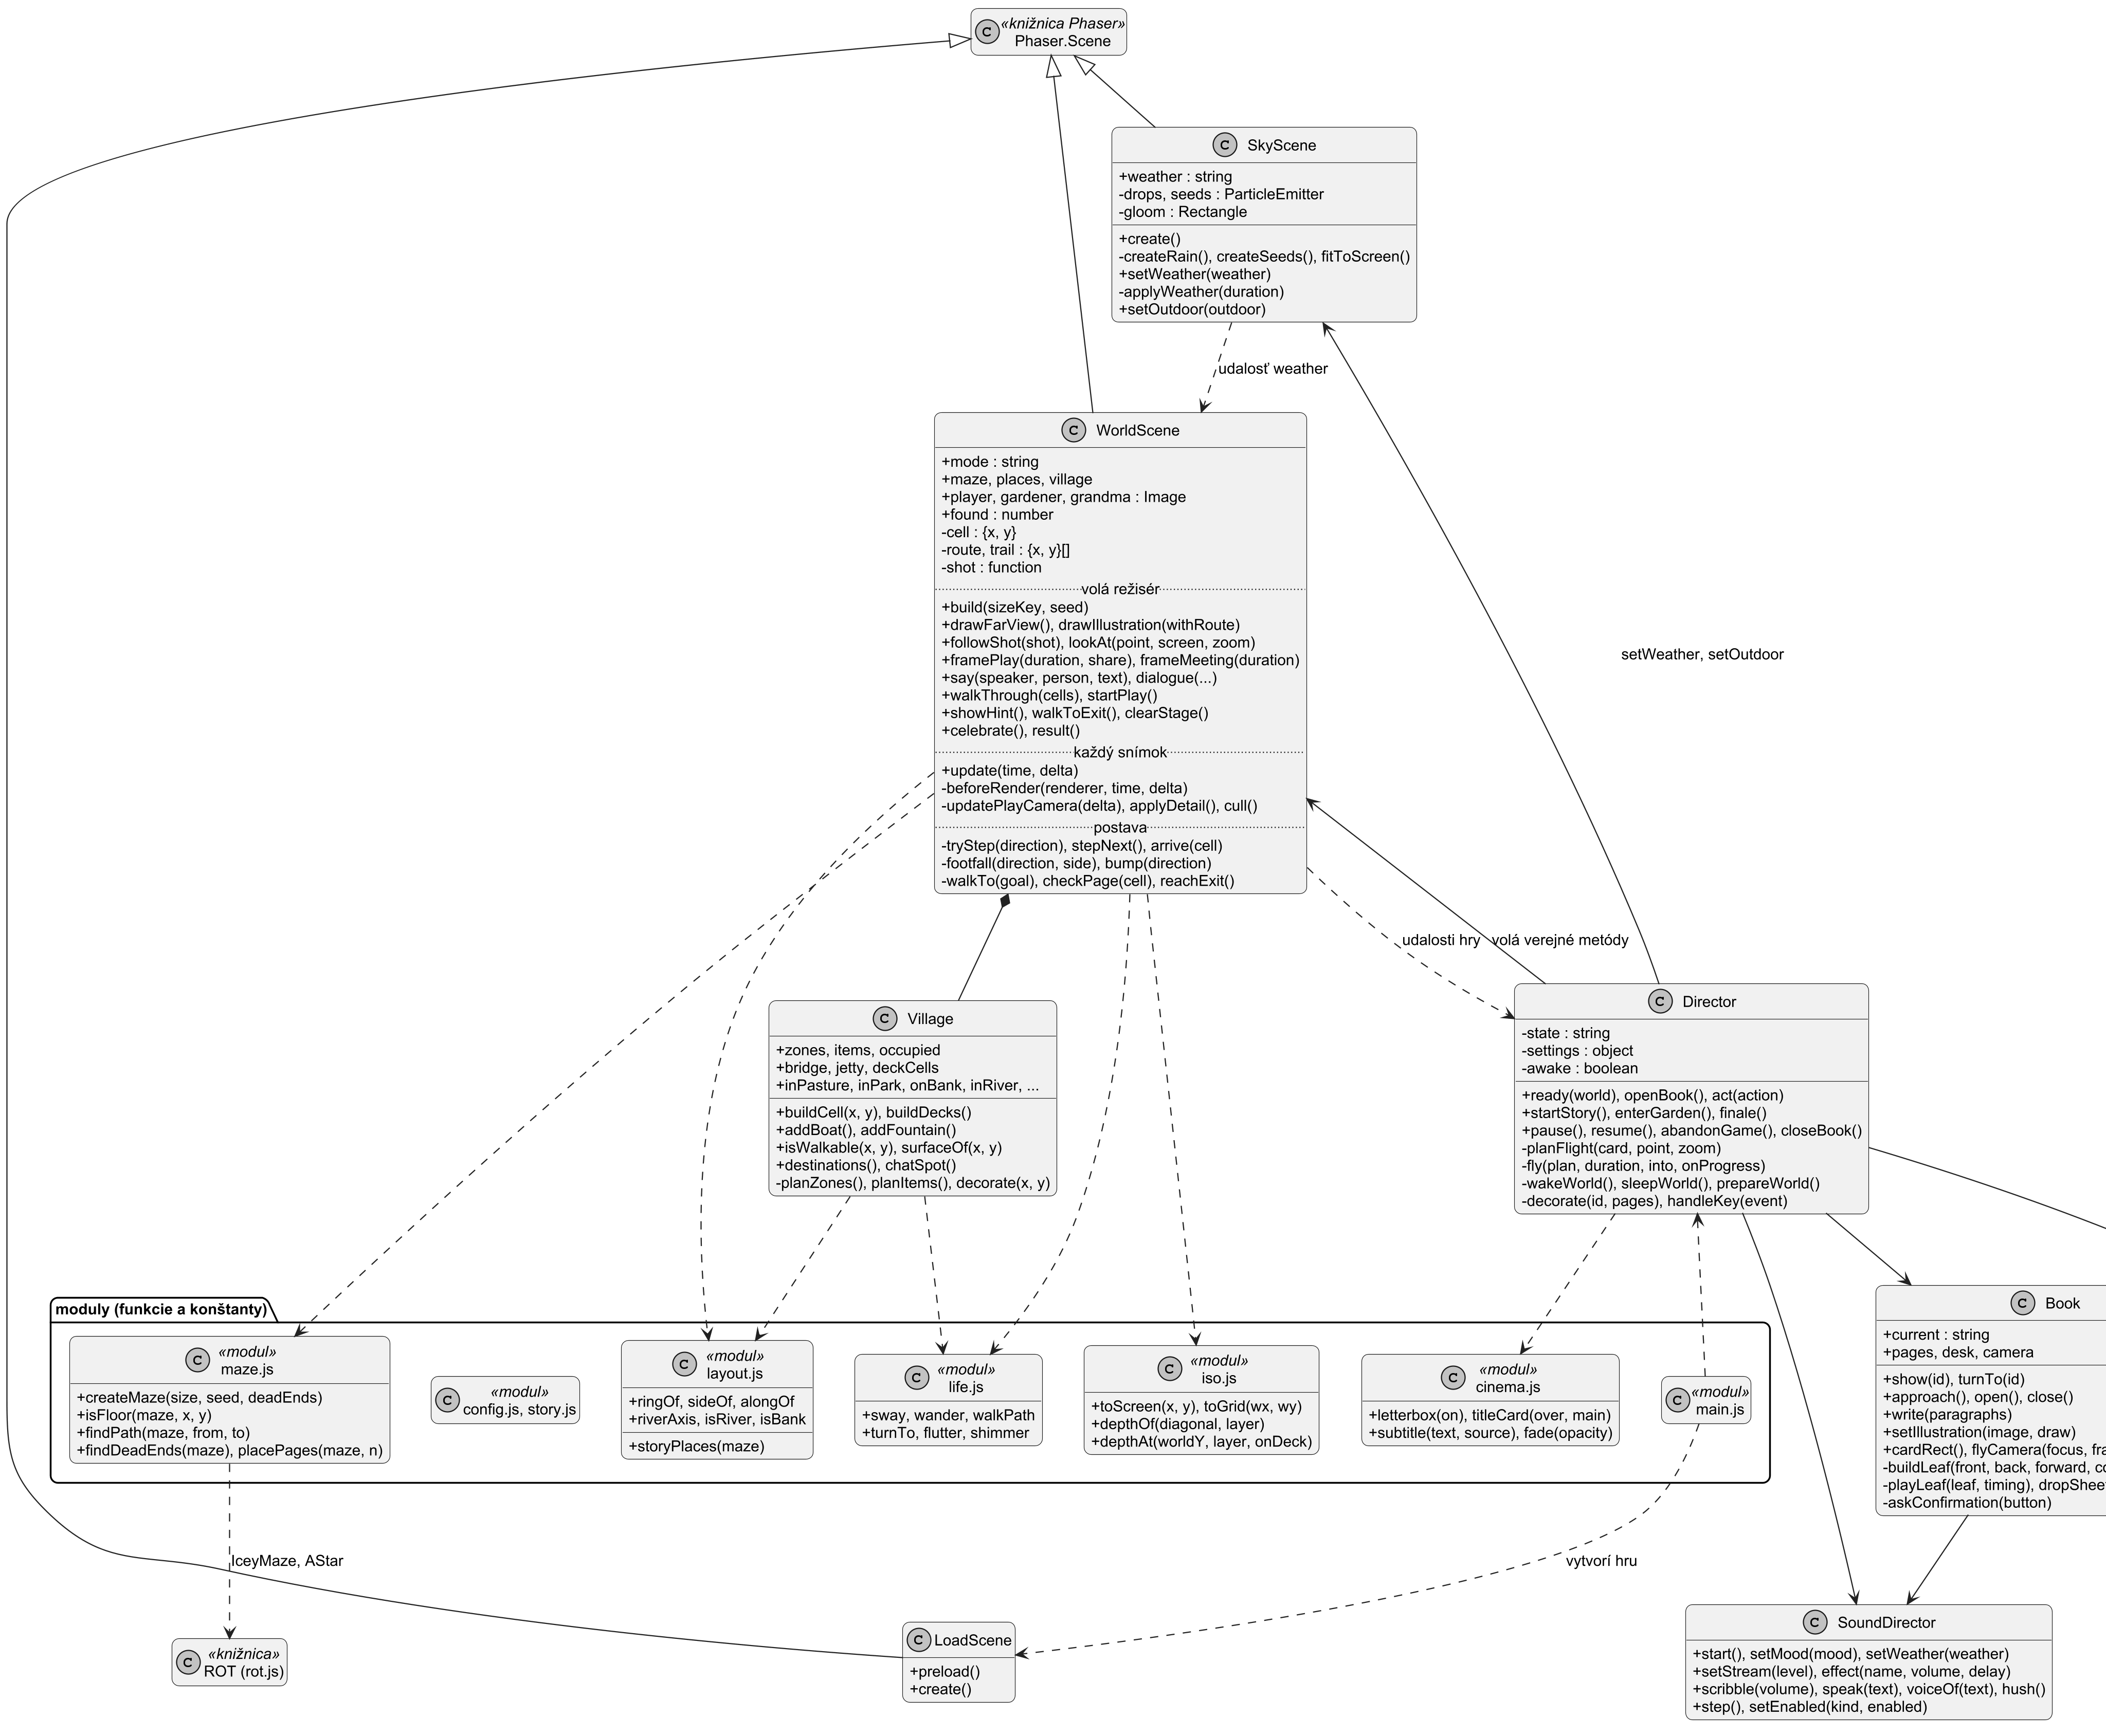
\includegraphics[width=\textwidth]{triedy.png}
  \caption{Diagram tried a modulov}\label{fig:triedy}
\end{figure}

\begin{figure}[H]
  \centering
  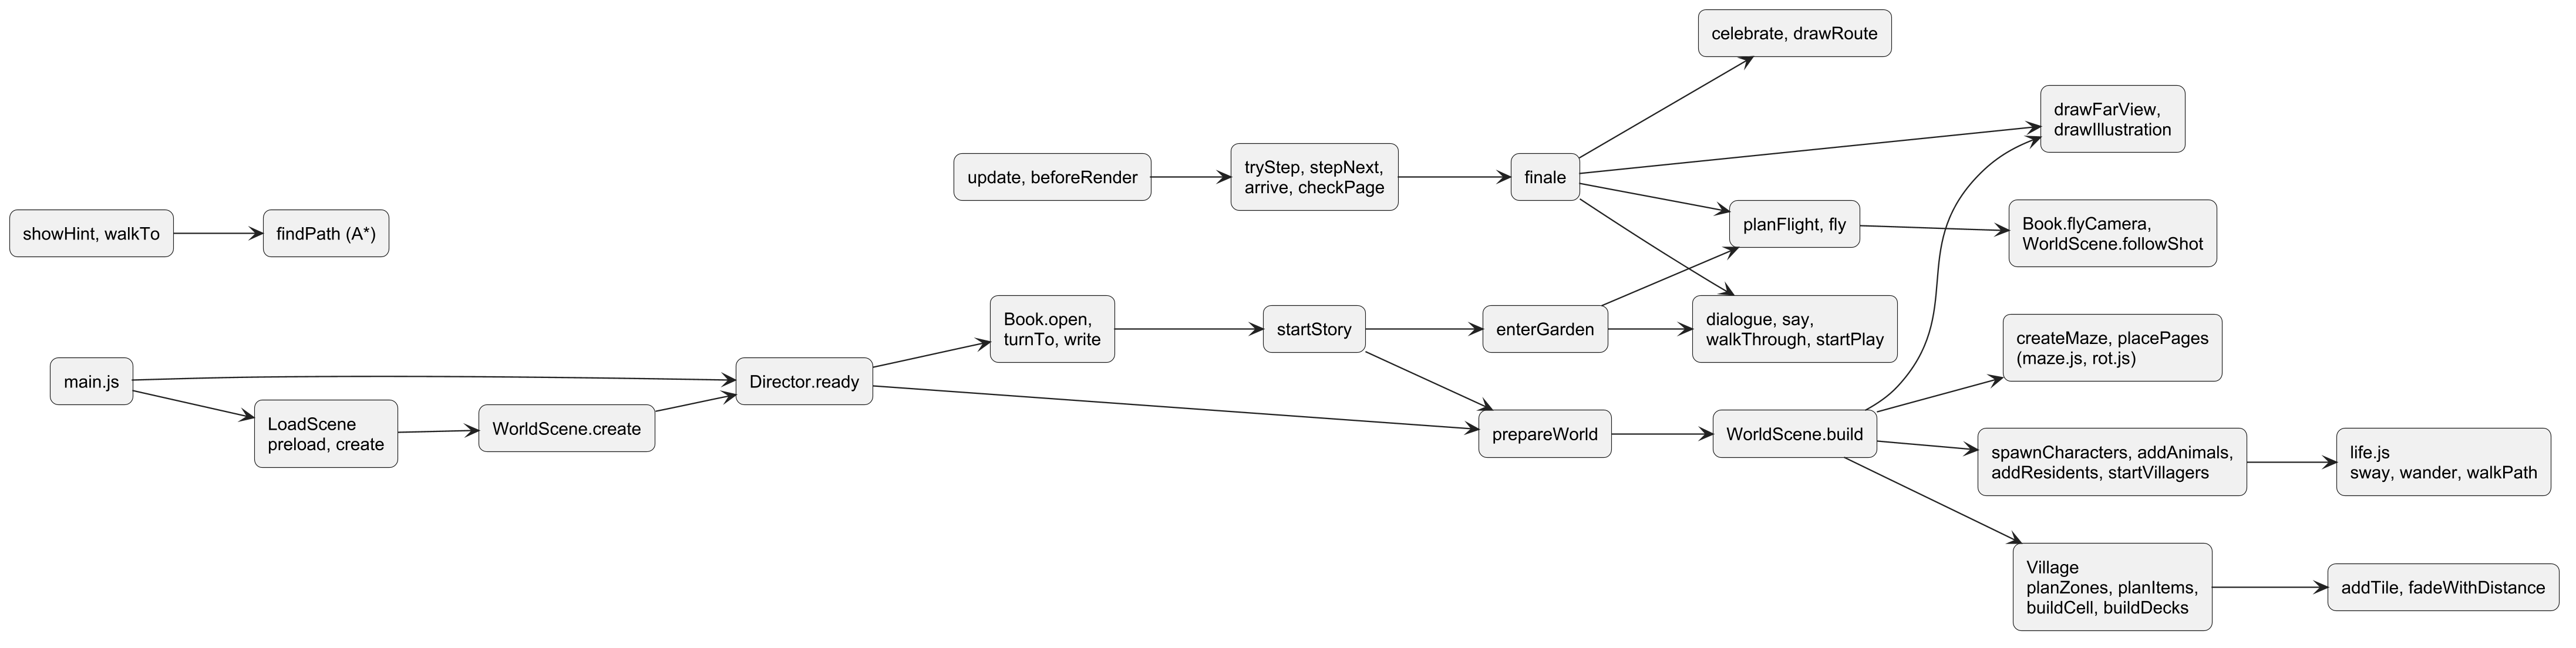
\includegraphics[width=\textwidth]{volania.png}
  \caption{Vnorenie volaní podprogramov}\label{fig:volania}
\end{figure}

\subsubsection{Moduly main.js, config.js, story.js, maze.js, iso.js, layout.js}
\begin{longtable}{@{}>{\raggedright\arraybackslash}p{0.34\textwidth}>{\raggedright\arraybackslash}p{0.61\textwidth}@{}}
  \toprule
  \textbf{Funkcia} & \textbf{Popis, vstup → výstup} \\ \midrule
  \endhead
  \subor{screenSize()} (main) & veľkosť okna v~pixeloch displeja → \subor{{width, height}} \\
  \subor{hasWebGL()} (main) & zistí podporu WebGL → \subor{boolean} \\
  (telo \subor{main.js}) & vytvorí \subor{Phaser.Game} so scénami, zvukovú réžiu a režiséra; pri zmene okna zmení veľkosť plátna \\
  \subor{STORY} (story) & všetky texty príbehu: prológ, rozhovory, spomienky, epilóg \\
  \subor{createMaze(size, seed, deadEnds)} & vygeneruje bludisko (ROT.Map.IceyMaze) s~aspoň \subor{deadEnds} slepými uličkami, otvorí vstup a bránu → objekt \subor{maze} \\
  \subor{isFloor(maze, x, y)} & je bunka voľná a vnútri mriežky? → \subor{boolean} \\
  \subor{findPath(maze, from, to)} & najkratšia cesta A* (4-okolie) → pole buniek bez počiatočnej, prázdne ak cesta neexistuje \\
  \subor{findDeadEnds(maze)} & miestnosti s~jediným voľným susedom → pole buniek \\
  \subor{placePages(maze, count)} & bunky zväzkov kresieb v~rovnomerne rozložených vzdialenostiach \\
  \subor{toScreen(x, y)}, \subor{toGrid(wx, wy)} & bunka ↔ svetové súradnice (rovnica~\ref{eq:iso}) \\
  \subor{depthOf(diagonal, layer)} & hĺbka pre maliarov algoritmus → číslo \\
  \subor{depthAt(worldY, layer, onDeck)} & hĺbka pohybujúceho sa objektu podľa polohy päty → číslo \\
  \subor{ringOf}, \subor{sideOf}, \subor{alongOf}, \subor{isRingCorner}, \subor{isLane} & poloha bunky voči bludisku (pás, strana, poradie) \\
  \subor{riverAxis}, \subor{isRiver}, \subor{isBank}, \subor{isBeyondRiver} & rieka a jej breh \\
  \subor{storyPlaces(maze)} & miesta príbehu: záhradník, babka, cesty k~vstupu a od brány, lampy \\ \bottomrule
\end{longtable}

\subsubsection{Trieda Director (director.js)}
\begin{longtable}{@{}>{\raggedright\arraybackslash}p{0.34\textwidth}>{\raggedright\arraybackslash}p{0.61\textwidth}@{}}
  \toprule
  \textbf{Metóda} & \textbf{Popis} \\ \midrule
  \endhead
  \subor{ready(world)} (+) & pod čiernou obrazovkou postaví svet a kresbu, zahreje grafickú kartu, uspí hru, ukáže stôl s~knihou \\
  \subor{openBook()} (+) & otvorí knihu (prvé kliknutie povolí zvuk) \\
  \subor{act(action)} (+) & akcie tlačidiel knihy (\subor{data-akcia}) \\
  \subor{decorate(id, pages)} & doplní texty, údaje o~ceste a stav nastavení do dvojstrany \\
  \subor{changeSetting(input)} & zmena nastavenia, uloženie do \subor{localStorage} \\
  \subor{wakeWorld()}, \subor{sleepWorld()} & prebudí / uspí hernú slučku a scény \\
  \subor{prepareWorld()} & postaví nový svet a nakreslí ho do knihy (vopred) \\
  \subor{planFlight(card, point, zoom)} & plán spoločného letu kamery knihy a sveta → \subor{{focus, at(u), clear, solid}} \\
  \subor{fly(plan, duration, into, onProgress)} & let podľa plánu; prebúdza a uspáva hru podľa priebehu \\
  \subor{startStory()}, \subor{enterGarden()} & prológ, let do kresby, rozhovor so záhradníkom, začiatok hry \\
  \subor{onPageFound(found)} & nájdený zväzok: lístok, dážď, titulky \\
  \subor{finale()} & babka, oslava, let do knihy, epilóg \\
  \subor{pause()}, \subor{resume()}, \subor{abandonGame()} & záložka, návrat do hry, zahodenie cesty \\
  \subor{closeBook()} & zavretie knihy a ukončenie aplikácie \\
  \subor{handleKey(event)} & Esc, Enter, medzerník, F \\ \bottomrule
\end{longtable}

\subsubsection{Trieda Book (book.js) a moduly cinema.js, hud.js, sound.js}
\begin{longtable}{@{}>{\raggedright\arraybackslash}p{0.34\textwidth}>{\raggedright\arraybackslash}p{0.61\textwidth}@{}}
  \toprule
  \textbf{Metóda / funkcia} & \textbf{Popis} \\ \midrule
  \endhead
  \subor{createPages()} & strany zo šablón so záhlavím a číslom strany \\
  \subor{show(id)}, \subor{turnTo(id)} (+) & ukáže dvojstranu / otočí listy k~nej (pri preskočení viacerých dvojstrán viac listov) → strany dvojstrany \\
  \subor{buildLeaf}, \subor{playLeaf}, \subor{dropSheets} & otáčaný list z~pásikov v~3D s~tieňmi, jeho animácia a zmiznutie otočených listov \\
  \subor{approach()}, \subor{open()}, \subor{close()} (+) & úvodný záber, otvorenie a zatvorenie dosky so zvukmi \\
  \subor{write(paragraphs)} (+) & písanie textu v~rytme rozprávača, ktorý text číta; kliknutie dopíše \\
  \subor{setIllustration(url, draw)} (+) & kresba sveta na stranu, vpíjanie do papiera \\
  \subor{cardRect()}, \subor{flyCamera(focus, frames, d)} (+) & poloha kresby, let kamery knihy (Web Animations) \\
  \subor{askConfirmation}, \subor{answerConfirmation} & potvrdenie nevratnej akcie na strane \\
  \subor{letterbox}, \subor{titleCard}, \subor{subtitle}, \subor{fade} (cinema) & filmové pásy, titulok kapitoly, titulky, zatmenie \\
  \subor{Hud.reset}, \subor{show}, \subor{setStatus}, \subor{collect} & lístok s~úlohou, čas a kroky, let zväzku na lístok \\
  \subor{SoundDirector.setMood}, \subor{setWeather}, \subor{effect}, \subor{step} & nálada (kniha, záhrada, pauza), počasie, efekty s~oneskorením, kroky \\
  \subor{scribble}, \subor{speak}, \subor{voiceOf}, \subor{hush} & slučka ceruzky s~hlasitosťou podľa hrotu; veta rozprávača či postavy (stíši hudbu), časy jej slov; doznenie reči a kreslenia \\ \bottomrule
\end{longtable}

\subsubsection{Triedy LoadScene, SkyScene a Village}
\begin{longtable}{@{}>{\raggedright\arraybackslash}p{0.34\textwidth}>{\raggedright\arraybackslash}p{0.61\textwidth}@{}}
  \toprule
  \textbf{Metóda} & \textbf{Popis} \\ \midrule
  \endhead
  \subor{LoadScene.preload()}, \subor{create()} & načítanie atlasu, textúr a zvukov; udalosti \subor{load-progress}, \subor{load-error} \\
  \subor{SkyScene.createRain()}, \subor{createSeeds()} & častice dažďa a semienok vo vetre \\
  \subor{setWeather(weather)}, \subor{applyWeather} & dážď a slnko s~plynulým prechodom, udalosť \subor{weather} \\
  \subor{setOutdoor(outdoor)}, \subor{gust()} & semienka iba v~záhrade; poryv vetra pri oslave \\
  \subor{Village.planZones()}, \subor{planItems()} & plán usadlosti \\
  \subor{buildCell(x, y)}, \subor{decorate(x, y)} & terén, cesta, predmet alebo príroda na bunke \\
  \subor{planDecks()}, \subor{buildDecks()}, \subor{addBoat()}, \subor{addFountain()} & most, mólo, loďka, fontána \\
  \subor{isWalkable(x, y)}, \subor{surfaceOf(x, y)} & kde smú chodiť ľudia, druh povrchu \\
  \subor{inPasture}, \subor{inPark}, \subor{onBank}, \subor{inRiver}, … & kde smú stáť zvieratá \\ \bottomrule
\end{longtable}

\subsubsection{Trieda WorldScene}
\begin{longtable}{@{}>{\raggedright\arraybackslash}p{0.34\textwidth}>{\raggedright\arraybackslash}p{0.61\textwidth}@{}}
  \toprule
  \textbf{Metóda} & \textbf{Popis} \\ \midrule
  \endhead
  \multicolumn{2}{@{}l}{\emph{volané režisérom (public)}} \\
  \subor{build(sizeKey, seed)} & bludisko, svet, postavy, život vo svete, obraz z~výšky \\
  \subor{drawFarView()}, \subor{drawIllustration(route)} & obraz ostrova do textúry; kresba do knihy → adresa obrázka \\
  \subor{followShot(shot)}, \subor{lookAt(p, s, z)} & kamera riadená funkciou času (spoločný let); kamera na bod \\
  \subor{framePlay}, \subor{frameMeeting} & let kamery na bludisko / na stretnutie s~babkou \\
  \subor{say}, \subor{writeLine}, \subor{dialogue}, \subor{placeBubble} & bublina: postava vetu povie, text sa píše v~rytme reči a bublina sa sama zavrie; rozhovor; bublina je vždy celá v~zábere (nad filmovými pásmi) \\
  \subor{walkThrough(cells)}, \subor{startPlay()} & filmová chôdza, začiatok hry \\
  \subor{showHint()}, \subor{walkToExit()} & nápoveda ceruzkou, ukážka riešenia \\
  \subor{greet()}, \subor{celebrate()}, \subor{clearStage()} & radosť pri babke, oslava s~kreslením cesty, voľný záber \\
  \subor{result()} & čas, kroky, najkratšia cesta, zväzky \\
  \multicolumn{2}{@{}l}{\emph{každý snímok}} \\
  \subor{update(time, delta)} & potok, kamera hry, čas, klávesy \\
  \subor{beforeRender}, \subor{applyDetail}, \subor{cull}, \subor{updateMargins}, \subor{seeThroughHedges} & spoločný záber, úroveň detailov, orezanie, okraje listu, priesvitné ploty pred postavou \\
  \multicolumn{2}{@{}l}{\emph{stavba a život sveta (private)}} \\
  \subor{buildMazeCell}, \subor{placeGates}, \subor{placeNooks}, \subor{placePages}, \subor{addTile} & bludisko, brány, ozdoby, zväzky, kresba na bunke \\
  \subor{spawnCharacters}, \subor{addResidents}, \subor{addAnimals}, \subor{addButterflies} & postavy príbehu, obyvatelia, zvieratá, motýle \\
  \subor{startVillagers}, \subor{sendVillager}, \subor{roadRoute} & chodci po cestách (A*) \\
  \subor{addWave}, \subor{addRipple}, \subor{scheduleBirds}, \subor{onWeather} & vlnky, kruhy na vode, vtáky, reakcia na počasie \\
  \multicolumn{2}{@{}l}{\emph{postava (private)}} \\
  \subor{tryStep}, \subor{stepNext}, \subor{arrive}, \subor{bump}, \subor{walkTo}, \subor{footfall} & pohyb postavy, stopy (diagram vyššie) \\
  \subor{checkPage}, \subor{reachExit} & zdvihnutie zväzku, dôjdenie k~bráne \\
  \subor{updateHover}, \subor{handlePointerUp}, \subor{handleWheel} & krúžok pod kurzorom (každý snímok), chôdza kliknutím, priblíženie \\
  \subor{drawRing}, \subor{eraseRing} & krúžok cieľa (kliknutie, brána) sa nakreslí, dýcha a rozplynie \\ \bottomrule
\end{longtable}

Udalosti, ktorými \subor{WorldScene} informuje režiséra: \subor{world-created}, \subor{hud-update},
\subor{first-move}, \subor{page-found}, \subor{reached-exit}; scéna \subor{LoadScene}:
\subor{load-progress}, \subor{load-error}; scéna \subor{SkyScene} oznamuje zmenu počasia
udalosťou \subor{weather}.

% =============================================================================
\section{Preklad programu}

\subsection{Zoznam zdrojových textov}

Zdrojové texty sú vypísané v~prílohe – dokumente Zdrojové texty.

\begin{table}[H]
  \centering
  \begin{tabularx}{\textwidth}{@{}>{\raggedright}p{0.4\textwidth}X@{}}
    \toprule
    \textbf{Súbor} & \textbf{Obsah} \\ \midrule
    \subor{index.html}, \subor{css/hra.css} & stôl, kniha a šablóny strán, filmová vrstva, údaje počas hry; vzhľad \\
    \subor{js/main.js}, \subor{js/config.js}, \subor{js/story.js} & vstupný bod, konštanty, texty príbehu \\
    \subor{js/director.js} & režisér – scenár aplikácie \\
    \subor{js/book.js}, \subor{js/cinema.js}, \subor{js/hud.js}, \subor{js/sound.js} & kniha, filmová vrstva, údaje počas hry, zvuky \\
    \subor{js/maze.js}, \subor{js/iso.js}, \subor{js/layout.js} & bludisko, izometrická projekcia, geometria sveta \\
    \subor{js/village.js}, \subor{js/life.js} & krajina usadlosti, správanie živých tvorov \\
    \subor{js/scenes/*.js} & scény LoadScene, WorldScene, SkyScene \\
    \subor{spustit.cmd} & spustenie lokálneho webového servera \\
    \subor{nastroje/atlas.js}, \subor{ui-textury.js}, \subor{snimky.js}, \subor{hlasy.py} & atlas kresieb, textúry knihy, snímky a video, hlasy \\ \bottomrule
  \end{tabularx}
\end{table}

\subsection{Požiadavky na technické prostriedky pri preklade}

Ľubovoľný osobný počítač s~4 GB RAM a 2 GB voľného miesta (nástroje Node.js, Playwright, TeX).

\subsection{Požiadavky na programové prostriedky pri preklade}

Program sa neprekladá – JavaScript vykonáva priamo prehliadač. Na úpravy postačuje textový
editor alebo WebStorm. Pre nástroje v~priečinku \subor{nastroje}: Node.js 20 alebo novší
a balíky \subor{sharp} (úprava obrázkov), \subor{free-tex-packer-core} (atlas textúr),
\subor{playwright} (snímky obrazovky a video, prehliadač Chrome); na kódovanie videa a hlasov
ffmpeg s~kodekmi x264, AAC a Vorbis (cesta v~premennej \subor{FFMPEG}); na hlasy Python~3,
pripojenie na internet a kľúč služby ElevenLabs v~premennej \subor{ELEVENLABS\_API\_KEY}. Pre dokumentáciu:
distribúcia TeX (XeLaTeX, biber, latexmk) a PlantUML (Java) pre diagramy.

\subsection{Vlastný preklad}

\begin{enumerate}
  \item Úprava programu: zmenený súbor sa uloží a stránka v~prehliadači sa obnoví (F5);
    server zo \subor{spustit.cmd} zakazuje vyrovnávaciu pamäť, takže sa načíta aktuálna verzia.
  \item Zmena zoznamu kresieb v~\subor{config.js}: v~priečinku \subor{nastroje} sa spustí
    \subor{npm install} (raz) a \subor{npm run atlas}; vznikne nový \subor{texture/mesto.png} a \subor{.json}.
  \item Zmena textúr knihy a rozhrania: \subor{npm run ui}.
  \item Zmena viet v~\subor{story.js}: \subor{npm run hlasy} (s~kľúčom v~\subor{ELEVENLABS\_API\_KEY}) – nahovorí
    všetky vety znova a zapíše časy slov do \subor{audio/hlas/hlasy.json}.
  \item Snímky a video do dokumentácie: \subor{npm run snimky} (len video: \subor{node snimky.js video}).
    Video sa hrá ako skutočná hra v~okne prehliadača mimo obrazovky – myš sa pohybuje ako ruka
    (zakrivená dráha, rozbeh a spomalenie, chvíľa nad cieľom) a nástroj do stránky pridá kurzor
    ceruzky, ktorý by nahrávanie inak nezachytilo. Nahráva sa karta so zvukom (MediaRecorder,
    H.264 kódované grafickou kartou, aby nahrávanie nebrzdilo hru); takmer priehľadná vrstva,
    ktorá sa mení každý snímok, zabráni, aby prehliadač pri zmene pohybu v~obraze na štvrť
    sekundy prestal posielať snímky. Nakoniec ffmpeg video zakóduje do H.264 s~konštantnou
    kvalitou a zjednotenou hlasitosťou.
  \item Diagramy: \subor{java -jar plantuml.jar -charset UTF-8 -tpng -o ../obrazky diagramy/*.puml}.
  \item Dokumentácia: v~priečinku \subor{dokumentacia} príkaz \subor{latexmk} (nastavenie
    v~\subor{.latexmkrc}) vytvorí tri PDF v~priečinku \subor{dist}.
  \item Balík na odovzdanie: z~koreňa repozitára sa spustí \subor{python nastroje/balik.py}.
    Vznikne \subor{Olym_PG1_20262027.zip} s~hrou a tromi príručkami; video do balíka nevstupuje.
\end{enumerate}

Vstupné kresby pre nástroje sú v~\subor{nastroje/podklady}; uložené sú iba použité podklady.
Repozitár obsahuje aj nastavenie GitLab CI: kontrolu syntaxe, zostavenie ZIP a nasadenie hry
na GitLab Pages. Pri spustení samotnej hry sa tieto nástroje nepoužívajú.

% =============================================================================
\section{Nadväznosť na iné programové produkty}

Aplikácia využíva webové technológie HTML5, CSS3 (transformácie v~3D, \subor{initial-letter},
masky), JavaScript (ECMAScript 2022, moduly ES), WebGL (cez knižnicu Phaser), Web Animations API
a Web Audio API. Nepoužíva databázu ani sieťovú komunikáciu; jediné uložené údaje sú
nastavenia v~\subor{localStorage} prehliadača.

% =============================================================================
\section{Zhodnotenie riešenia}

Splnené ciele: generovanie bludiska, pohyb klávesnicou aj myšou, nápoveda a ukážka riešenia
algoritmom A*, izometrické zobrazenie s~maliarovým algoritmom, papier a vzdušná perspektíva
miešaním farieb, živý svet, kniha ako menu so stranami, ktoré sa otáčajú ako papier, filmové
prechody s~jedným nepretržitým letom kamery, titulná strana a potvrdenie nevratných akcií podľa
pokynov. Vlastný kód má približne 4\,900 riadkov JavaScriptu (s~HTML a CSS asi 6\,200, vrátane
komentárov); všetky kresby, zvuky a knižnice sú prevzaté a uvedené v~literatúre. Plynulosť sa
merala na integrovanej grafike Intel UHD Graphics 630 pri 1920 × 1080: kniha, lety kamery aj hra
bežia pri 59 až 60 snímkach za sekundu.

Obmedzenia a možnosti ďalšieho vývoja:
\begin{itemize}
  \item rozohraná cesta sa neukladá; bolo by možné uložiť semienko a polohu postavy,
  \item tabuľka najlepších výsledkov pre jednotlivé veľkosti bludiska,
  \item dotykové ovládanie pre tablety,
  \item postavy majú jednu pózu (kresby balíka nemajú animáciu chôdze); chôdzu naznačuje pohyb
    celej kresby,
  \item ďalšie kapitoly príbehu v~iných častiach usadlosti.
\end{itemize}

% =============================================================================
\printbibliography[heading=bibnumbered, title={Zoznam použitej literatúry}]

% =============================================================================
\section{Zoznam príloh}

\begin{enumerate}[label=Príloha \Alph*:, leftmargin=*]
  \item Zdrojové texty – samostatný dokument \subor{Zdrojove_texty.pdf}.
  \item Zdrojové súbory diagramov (PlantUML) – priečinok \subor{diagramy} v~zdrojoch dokumentácie.
\end{enumerate}

\end{document}
